% arara: xelatex
% arara: biber
% arara: xelatex: { synctex: true }

\documentclass[12pt,a4paper,oneside,final]{report}

\usepackage{listings}
\lstdefinelanguage{G2}{
  keywords={when,the,value,of,as,of,seconds,ago,rate,of,change,per,second,during,the,last,second,seconds,then,conclude,that,disease_diagnosis,deficiency_diagnosis,nutrition_state,recommendation,every,melon_plant,melon_field,display_object},
  literate={\textquotedblleft}{"}1
           {\textquotedblright}{"}1,
  morestring=[b]",
  comment=[l]%
}
\usepackage{polyglossia}
\setmainlanguage{russian}
\usepackage{siunitx}
\sisetup{
  detect-all,
  locale = DE, % DE использует запятую как десятичный разделитель, что ближе к RU
  range-phrase = {--},
  range-units = single
}
\usepackage{float}

\input{chapters/thesis-template-macro.tex}


\usepackage[
  style=gost-numeric,
  sorting=none,
  language=auto,
  autolang=other
]{biblatex}
\addbibresource{chapters/biblio.bib}

\begin{document}

% Для вставки бланка титульного листа из PDF-файла
%\includepdf[pages={-}, offset=0mm -0mm]{chapters/pz_vkr_bakalavry.pdf}

% Для титульного листа, сверстанного в LaTeX
\thispagestyle{empty}
\input{title/blank-header}

\vfill

\begin{center}
  Направление подготовки 09.04.04 Программная инженерия

  \vfill

  {\Large{\textbf{Пояснительная записка}}}

  к \theprojecttypefulldative\space студентов на тему:

  {\Large\thetitle}
\end{center}

\vfill

{\large

\noindent
\begin{tabularx}{\linewidth}{@{}l>{\centering}XlX@{}}
Группа              & \raggedright\groupOne &                & \\ 
                    & \raggedright\groupTwo &                & \\ 
Студент             & \theauthorpzapproval        & \theauthor     & \\ \hhline{~-~}
Руководитель        & \thesupervisorpzapproval    & \thesupervisor & \\ \hhline{~-~}
\end{tabularx}

\vfill

\noindent
\begin{tabularx}{\linewidth}{@{}l>{\centering}XX@{}}
Оценка руководителя & \thesupervisorpzgrade & \\ \hhline{~-}
\end{tabularx}

\begin{center}
\textbf{Москва \the\year}
\end{center}

}

%%% Local Variables:
%%% TeX-engine: xetex
%%% eval: (setq-local TeX-master (concat "../" (seq-find (-cut string-match ".*-3-pz\.tex$" <>) (directory-files ".."))))
%%% End:

\newpage
\clearpage
\tableofcontents
\clearpage

\chapter{Исследование проблемной области "Процесс диагностики заболеваний дынь"}
\label{chapter1}

\section{Краткая характеристика источников знаний и методов получения знаний}

Для моделирования понятийной структуры проблемной области используются три основные категории источников знаний:
\begin{itemize}
    \item люди и эксперты, обладающие глубокими знаниями и опытом в соответствующей области;
    \item разнообразные литературные источники, включая книги, справочники, инструкции и прочие печатные материалы;
    \item базы данных, электронные носители и иные цифровые ресурсы.
\end{itemize}
В рамках данной работы в качестве источника знаний использовалась литература (источник второго типа). В частности, основой послужили труды профессора, доктора технических наук Г.В. Рыбиной: книга «Теория и технология построения интегрированных экспертных систем» и совместное издание с С.С. Параджановым «Технология построения динамических интеллектуальных систем». Эти материалы применялись непосредственно при разработке и конструировании прототипа динамической интегрированной экспертной системы.  Для тематической части- книга Кярыма Маметгулова, Бахрии Юсубовой ”Болезни бахчевых культур и меры борьбы против них”

\section{Глоссарий предметной области}

\begin{description}
    \item[Сад] участок земли с растениями, выращиваемыми в открытом грунте или защищённом пространстве для получения урожая.
    \item[Датчик] устройство для преобразования параметров окружающей среды в измеримые сигналы, пригодные для анализа и обработки информации.
    \item[Воздух] газовая смесь, в составе которой преобладают азот и кислород, образующие земную атмосферу.
    \item[Благоприятные условия воздуха] такой состав атмосферы, при котором растения могут длительное время развиваться и функционировать оптимально.
    \item[Температурный режим воздуха] количественное измерение степени нагрева или охлаждения атмосферного воздуха.
    \item[Влажность атмосферы] степень присутствия водяных паров в воздухе, влияющая на жизнедеятельность растений.
    \item[Почва] верхний плодородный слой земной коры, состоящий из органических и минеральных компонентов, жидкостей и газов, обеспечивающих развитие растительных организмов.
    \item[Влажность грунта] процентное содержание воды в почве относительно её полностью высушенной массы или на единицу объёма.
    \item[Содержание азотных компонентов] уровень концентрации азота в почвенной среде, необходимый для растений.
    \item[Содержание калийных компонентов] количество калия в почве, влияющего на обменные процессы и устойчивость культур.
    \item[Природная среда] совокупность физических, химических и биологических факторов, в которых развиваются растения.
    \item[Специалист по растениеводству] лицо с профессиональной подготовкой и опытом в области выращивания и ухода за культурами.
    \item[Визуальная диагностика] метод определения заболеваний и дефицитов по внешним признакам и изменениям внешнего вида растений.
    \item[Микроэлементы и макроэлементы] химические вещества, необходимые растениям для полноценного роста и развития.
    \item[Симптомы заболевания] видимые изменения структуры и окраски растения, указывающие на наличие болезни или стресса.
    \item[Динамическое содержание питательных веществ] колебание уровня элементов питания в почве с течением времени и сезонов.
    \item[Дыня (Cucumis melo)] культура из семейства тыквенных, характеризующаяся мясистыми плодами и требующая специального ухода при выращивании.
    \item[Мучнистая роса] грибковое поражение надземных частей растения, проявляющееся образованием светлого налёта на листовых пластинках и стеблях.
    \item[Фузариозное увядание] болезнь, вызванная грибковым возбудителем, приводящая к потере тургора и отмиранию растительной ткани.
    \item[Антракноз] грибковая инфекция, характеризующаяся формированием некротических пятен тёмного цвета на листьях и плодах с последующей гнилью.
    \item[Вредоносные организмы] живые существа, способные причинять вред растительным культурам и служить переносчиками инфекций.
\end{description}

\section{Описание задач/подзадач, решаемых в данной предметной области}

В настоящее время проблемой своевременной диагностики и предотвращения заболеваний занимается специалист по защите растений. Для эффективного выявления болезней дынь и оценки состояния растений при изменяющихся условиях питания необходима полная и достоверная информация о визуальных симптомах заболеваний, соответствующих характеру поражения. Данная задача является сложной для специалиста и требует постоянного анализа состояния культур и внешних факторов, влияющих на их здоровье. Высокая вариабельность проявления симптомов в условиях нестабильного содержания питательных веществ в почве усложняет процесс идентификации болезней и выбора адекватных мер борьбы. Для успешного выполнения диагностических и профилактических работ необходимо поставить и решить следующие задачи.

\subsection{Задача мониторинга}

Система в реальном времени получает визуальные данные о состоянии листьев и плодов дынь, информацию о содержании питательных веществ в почве и климатических параметрах окружающей среды, фиксирует изменения окраски, появление пятен, деформации и других визуальных признаков, сигнализируя о возможном развитии заболевания или дефицита элементов питания.
Постановка задачи:
Дано: Данные о визуальных признаках растений дынь (цвет листьев, наличие пятен, состояние плодов), показатели содержания азота, фосфора, калия, кальция и магния в почве, метеорологические данные (температура, влажность, освещённость).
Требуется: Отслеживать текущее состояние дынь в условиях нестабильного содержания питательных веществ и оповещать о появлении подозрительных визуальных симптомов, указывающих на развитие заболевания.

\subsection{Задача диагностики}

Система анализирует визуальные признаки поражённых растений дынь (характер пятен, налёты, деформации, изменение окраски листьев и плодов), соотносит выявленные симптомы с известными болезнями и дефицитами питательных веществ, определяет вероятный диагноз и предлагает рекомендации по лечению и профилактике на основе анализа условий выращивания.
Постановка задачи:
Дано: Визуальные данные о симптомах поражения дынь (фотографии, описание признаков), информация о содержании макро- и микроэлементов в почве, условиях выращивания (температура, влажность, освещённость).
Требуется: Определить вид заболевания или тип дефицита питательных веществ и сформировать набор рекомендаций по устранению выявленной проблемы с учётом текущих условий окружающей среды.

\section{Описание внешнего мира - сада с дынями}

Внешний мир сада, в котором выращиваются дыни, включает в себя природные факторы (атмосферные осадки, температурные колебания, солнечное излучение, ветровые потоки) и антропогенные воздействия (применение удобрений, использование пестицидов, механическое воздействие). Их влияние обусловлено физическими, химическими и биологическими процессами, протекающими в почве и атмосфере.
Так, например, интенсивные осадки повышают влажность почвы и могут привести к вымыванию питательных веществ, что способствует их нестабильному содержанию в грунте. Недостаток осадков, напротив, снижает доступность микроэлементов и может вызвать дефицит питания у растений. Повышение температуры воздуха ускоряет развитие грибковых заболеваний, таких как мучнистая роса, в то время как перепады влажности создают благоприятные условия для распространения патогенов.
Содержание азота, фосфора и калия в почве непрерывно изменяется под воздействием погодных условий, жизнедеятельности микроорганизмов и процессов выщелачивания. Эти колебания напрямую влияют на визуальное состояние растений, проявляясь в изменении окраски листьев, деформации побегов и снижении устойчивости к болезням.
Схематично взаимодействие сада и внешнего мира отражено на схеме, где дыни выступают системой, подвергающейся влиянию переменчивых условий окружающей среды и требующей постоянного мониторинга и диагностики состояния.

\section{Системный анализ на применимость технологии систем, основанных на знаниях}
Диагностика состояния сложных систем, таких как бахчевые культуры, основывается на анализе качественных данных (символов), а не на простых числовых расчетах. Эксперты считают эту задачу нетривиальной из-за множества входных параметров от датчиков и отсутствия прямого алгоритмического решения. Тем не менее, масштабы задачи позволяют эффективно использовать компьютерные системы. Таким образом, разработка интегрированной экспертной системы для этой предметной области является целесообразной.

Внедрение такой системы позволит значительно сократить расходы на обучение персонала и уменьшить количество специалистов, контролирующих состояние культур, а также объём специализированного оборудования. Следовательно, создание интегрированной экспертной системы экономически оправдано.

Решение этой задачи требует интеллектуального подхода и рассуждений, а не механических действий. Специалисты в данной области обладают знаниями о методах работы и согласны в подходах к решению, что подтверждает возможность создания интегрированной экспертной системы.

Исходя из вышеизложенного, применение методов и технологий динамических интегрированных экспертных систем в данной предметной области является обоснованным, уместным и оправданным.

\section{Постановка задачи}
Основной целью данной работы является создание прототипа динамической интегрированной экспертной системы (ИЭС). Эта система должна визуализировать текущие условия на поле и формировать диагностические заключения о состоянии культур, чтобы помочь агрономам оперативно принимать обоснованные решения.

\chapter{Моделирование проблемной области}
\label{chapter2}

\section{Построение фрагмента поля знаний на естественном языке}

В данном разделе приводится фрагмент полуформализованного описания проблемной области (фрагменты поля знаний) в виде совокупности конструкций вида: \enquote{ЕСЛИ \dots{} ТО \dots{}} на естественном языке, полученное в результате исследования данной проблемной области.

\begin{enumerate}
    \item Если на листьях появились жёлто-зелёные угловатые пятна и наблюдается серо-фиолетовый налёт на нижней стороне листьев, и влажность воздуха выше \SI{80}{\percent}, и температура воздуха ниже \SI{20}{\degree C}, то диагностировать \enquote{пероноспороз}.

    \item Если на стеблях и листьях наблюдается белый мучнистый налёт и листья закручиваются и становятся коричневыми, и влажность воздуха не менее \SI{50}{\percent}, и температура воздуха в диапазоне \SIrange{15}{25}{\degree C}, то диагностировать \enquote{мучнистая роса}.

    \item Если на нижней стороне листьев появился белый налёт, и влажность воздуха не менее \SI{50}{\percent}, и температура воздуха в диапазоне \SIrange{15}{25}{\degree C}, то диагностировать \enquote{мучнистая роса}.

    \item Если на нижней стороне листьев наблюдается серый налёт, и влажность воздуха выше \SI{80}{\percent}, и температура воздуха ниже \SI{20}{\degree C}, то диагностировать \enquote{ложная мучнистая роса (пероноспороз)}.

    \item Если на листьях появились жёлто-коричневые пятна с чёткой каймой и на стеблях образовались вдавленные овальные язвочки жёлто-коричневого цвета, и температура воздуха не менее \SI{20}{\degree C}, и влажность воздуха не менее \SI{80}{\percent}, то диагностировать \enquote{антракноз}.

    \item Если на листьях появились обширные пятна, и температура воздуха не менее \SI{20}{\degree C}, и влажность воздуха не менее \SI{80}{\percent}, то диагностировать \enquote{антракноз}.

    \item Если растение увядает, и листья желтеют от основания к верхушке, и корневая шейка темнеет, то диагностировать \enquote{фузариозное увядание}.

    \item Если растение увядает сильно и корни приобретают чёрный цвет, то диагностировать \enquote{фузариоз}.

    \item Если нижние листья становятся бледно-зелёными и содержание азота в почве критическое (уровень 0) и рост растения замедляется, то диагностировать \enquote{дефицит азота}.

    \item Если листья полностью пожелтели и содержание азота в почве менее 50 мг/кг, то диагностировать \enquote{дефицит азота}.

    \item Если листья приобретают тёмно-зелёную окраску с фиолетовым оттенком и содержание фосфора в почве критическое (уровень 0), то диагностировать \enquote{дефицит фосфора}.

    \item Если края листьев буреют и появляется краевой ожог и содержание калия в почве критическое (уровень 0), то диагностировать \enquote{дефицит калия}.

    \item Если между жилками старых листьев развивается хлороз и содержание магния в почве неоптимально (уровень 1), то диагностировать \enquote{дефицит магния}.

    \item Если между жилками старых листьев развивается интенсивный хлороз и содержание магния в почве менее 50 мг/кг и pH почвы щелочной (выше 7.5), то диагностировать \enquote{дефицит магния}.

    \item Если между жилками молодых листьев развивается хлороз и содержание железа в почве критическое (уровень 0), то диагностировать \enquote{дефицит железа}.

    \item Если между жилками молодых листьев развивается интенсивный хлороз и содержание железа в почве менее 10 мг/кг и pH почвы щелочной (выше 7.5), то диагностировать \enquote{дефицит железа}.

    \item Если листья сильно закручиваются и содержание магния в почве критическое (уровень 0), то диагностировать \enquote{тяжёлый дефицит магния}.

    \item Если жилки листьев зеленоватые и содержание магния в почве неоптимально (уровень 1), то диагностировать \enquote{лёгкий дефицит магния}.

    \item Если лист зелёный и на нём отсутствуют пятна, то состояние листа \enquote{здоровое}.

    \item Если лист жёлтый и на нём появились коричневые круглые пятна, то состояние листа \enquote{подозрение на заболевание}.

    \item Если лист имеет мучнистую текстуру и покрыт белым налётом, то состояние листа \enquote{обнаружена мучнистая роса}.

    \item Если края листа некротизированы (бурые) и текстура листа хрупкая, то состояние листа \enquote{тяжёлый дефицит питательных веществ}.

    \item Если нижняя сторона листа покрыта серым налётом и лист бледно-жёлтый, то состояние листа \enquote{обнаружена ложная мучнистая роса}.

    \item Если между жилками листа развивается хлороз (обесцвечивание) и жилки остаются зелёными, то состояние листа \enquote{дефицит микроэлементов}.

    \item Если на листе появились жёлтые пятна с жёлтым ореолом и пятна имеют концентрические кольца, то состояние листа \enquote{обнаружен антракноз}.

    \item Если лист увядает и приобретает тёмно-коричневый цвет, то состояние листа \enquote{подозрение на фузариоз}.

    \item Если лист имеет высокую влажность (покрыт росой) и воздух имеет высокую влажность и текстура листа мягкая, то состояние листа \enquote{риск грибковой инфекции}.

    \item Если лист старый и его цвет бледный, то состояние листа \enquote{нормальное старение}.

    \item Если высота растения нормальная и листья здоровые и стебель прочный, то состояние растения \enquote{активный рост}.

    \item Если высота растения остаётся позади в развитии и листья пожелтели, то состояние растения \enquote{наличие дефицита питательных веществ}.

    \item Если растение сильно увядает и стебель мягкий и корни чёрного цвета, то состояние растения \enquote{критическое корневое заболевание}.

    \item Если диагностирована мучнистая роса и состояние листа \enquote{обнаружена мучнистая роса}, то состояние растения \enquote{грибковое заболевание}.

    \item Если диагностирован антракноз и на листьях обширные пятна, то состояние растения \enquote{тяжёлое заболевание}.

    \item Если диагностирован дефицит азота и содержание азота в почве критическое, то состояние растения \enquote{азотное голодание}.

    \item Если высота растения нормальная и листья здоровые и состояние почвы отличное, то состояние растения \enquote{оптимальный рост}.

    \item Если на стебле присутствуют поражения (язвочки) и стебель бурый и обесцвечен, то состояние растения \enquote{стеблевое заболевание}.

    \item Если плод деформирован и диагностирован фузариоз, то состояние растения \enquote{нарушение плодоношения}.

    \item Если влажность почвы выше нормы (уровень 2) и содержание калия оптимально (уровень \geq 1) и содержание азота оптимально (уровень \geq 1), то состояние почвы \enquote{удовлетворительное}.

    \item Если влажность почвы высокая (уровень 2) и содержание калия оптимально (уровень 2) и содержание азота оптимально (уровень 2) и содержание магния оптимально (уровень 2), то состояние почвы \enquote{отличное}.

    \item Если влажность почвы высокая (уровень 2) и содержание магния неоптимально (уровень 1) и содержание азота оптимально (уровень 2), то состояние почвы \enquote{хорошее}.

    \item Если влажность почвы высокая (уровень 2) и содержание калия оптимально (уровень 2) и содержание азота неоптимально (уровень 1), то состояние почвы \enquote{хорошее}.

    \item Если влажность почвы низкая (уровень 0) и содержание калия оптимально (уровень 2) и содержание азота оптимально (уровень 2), то состояние почвы \enquote{удовлетворительное}.

    \item Если влажность почвы высокая (уровень 2) и содержание калия критическое (уровень 0) и содержание азота критическое (уровень 0) и содержание магния критическое (уровень 0), то состояние почвы \enquote{удовлетворительное}.

    \item Если влажность почвы высокая (уровень 2) и содержание азота критическое (уровень 0), то состояние почвы \enquote{неудовлетворительное}.

    \item Если влажность почвы высокая (уровень 2) и содержание магния критическое (уровень 0), то состояние почвы \enquote{неудовлетворительное}.

    \item Если влажность почвы низкая или критическая (уровень \leq 1) и содержание калия критическое (уровень 0) и содержание азота критическое (уровень 0) и содержание магния критическое (уровень 0), то состояние почвы \enquote{неудовлетворительное}.

    \item Если температура воздуха критическая (уровень 0) и влажность воздуха критическая (уровень 0), то состояние воздуха \enquote{критическое}.

    \item Если температура воздуха неоптимальная (уровень 1) и влажность воздуха оптимальна (уровень 2), то состояние воздуха \enquote{благоприятное}.

    \item Если температура воздуха оптимальна (уровень 2) и влажность воздуха оптимальна (уровень 2), то состояние воздуха \enquote{очень благоприятное}.

    \item Если содержание азота в почве критическое (уровень 0) и влажность почвы выше нормы (уровень 1), то состояние питания \enquote{критическое с риском вымывания}.

    \item Если содержание азота в почве неоптимально (уровень 1) и содержание калия в почве неоптимально (уровень 1) и содержание фосфора в почве неоптимально (уровень 1), то состояние питания \enquote{нестабильное}.

    \item Если содержание азота в почве оптимально (уровень 2) и содержание калия в почве оптимально (уровень 2) и содержание фосфора в почве оптимально (уровень 2), то состояние питания \enquote{стабильное}.

    \item Если диагностирована мучнистая роса и влажность воздуха высокая и температура воздуха умеренная (\SIrange{16}{20}{\degree C}), то выдать рекомендацию \enquote{обработать посадки коллоидной серой, соблюдать севооборот}.

    \item Если диагностирован пероноспороз и влажность почвы выше нормы (уровень 1), то выдать рекомендацию \enquote{обработать бордоской жидкостью, прогреть семена при \SI{45}{\degree C} в течение 2 часов}.

    \item Если диагностирован антракноз и температура воздуха высокая (\SIrange{24}{25}{\degree C}) и влажность воздуха выше \SI{60}{\percent}, то выдать рекомендацию \enquote{удалить пораженные части растений, обработать фунгицидами}.

    \item Если диагностировано фузариозное увядание, то выдать рекомендацию \enquote{удалить пораженные растения, продезинфицировать почву, соблюдать севооборот минимум 4 года}.

    \item Если диагностирован фузариоз, то выдать рекомендацию \enquote{удалить пораженные растения, продезинфицировать почву, избегать избыточной влажности}.

    \item Если диагностирована ложная мучнистая роса, то выдать рекомендацию \enquote{обработать медьсодержащими фунгицидами, улучшить вентиляцию, снизить влажность}.

    \item Если диагностирован дефицит азота и состояние питания нестабильное, то выдать рекомендацию \enquote{внести азотные удобрения (мочевина, аммиачная селитра), провести листовую подкормку 2\% раствором нитрата кальция}.

    \item Если диагностирован дефицит калия и содержание калия в почве критическое (уровень 0), то выдать рекомендацию \enquote{внести калийные удобрения, избегать избыточного азотного питания}.

    \item Если диагностирован дефицит магния, то выдать рекомендацию \enquote{провести внекорневую подкормку сульфатом магния}.

    \item Если диагностирован тяжёлый дефицит магния, то выдать рекомендацию \enquote{срочная внекорневая подкормка сульфатом магния 10\% раствором}.

    \item Если диагностирован лёгкий дефицит магния, то выдать рекомендацию \enquote{внекорневая подкормка сульфатом магния 5\% раствором, внесение органических удобрений}.

    \item Если диагностирован дефицит железа и pH почвы выше 7.5, то выдать рекомендацию \enquote{провести внекорневую подкормку хелатом железа, снизить pH почвы}.

    \item Если диагностирован дефицит фосфора, то выдать рекомендацию \enquote{внести фосфорные удобрения, улучшить усвояемость путем внесения органических удобрений}.
\end{enumerate}


\subsection{Правила на языке представления знаний системы G2}

\begin{lstlisting}[language=C, breaklines=true, breakatwhitespace=false]
unconditionally start detect_magnesium_deficiency(leaf1, soil1, plant1)
unconditionally start show_lights()
unconditionally start show_lights_diagnoz(plant1, air1, soil1)
unconditionally start constraints(air1, soil1, plant1)
unconditionally start simulate_day(air1, soil1, plant1)
initially start initialize_simulation()
    
for any soil soil1
    when the soil_humidity_state of soil1 = 1
    and the soil_potassium_state of soil1 >= 1
    and the soil_nitrogen_state of soil1 >= 1
    then conclude that the soil_state of soil1 = "satisfactory"

for any soil soil1
    when the soil_humidity_state of soil1 = 2
    and the soil_potassium_state of soil1 = 2
    and the soil_nitrogen_state of soil1 = 2
    and the soil_magnesium_state of soil1 = 2
    then conclude that the soil_state of soil1 = "excellent"

for any soil soil1
    when the soil_humidity_state of soil1 = 2
    and the soil_magnesium_state of soil1 = 1
    and the soil_nitrogen_state of soil1 = 2
    then conclude that the soil_state of soil1 = "good"

for any soil soil1
    when the soil_humidity_state of soil1 = 2
    and the soil_potassium_state of soil1 = 2
    and the soil_nitrogen_state of soil1 = 1
    then conclude that the soil_state of soil1 = "good"

for any soil soil1
    when the soil_humidity_state of soil1 = 0
    and the soil_potassium_state of soil1 = 2
    and the soil_nitrogen_state of soil1 = 2
    then conclude that the soil_state of soil1 = "satisfactory"

for any soil soil1
    when the soil_humidity_state of soil1 = 2
    and the soil_potassium_state of soil1 = 0
    and the soil_nitrogen_state of soil1 = 0
    and the soil_magnesium_state of soil1 = 0
    then conclude that the soil_state of soil1 = "satisfactory"

for any soil soil1
    when the soil_humidity_state of soil1 = 2
    and the soil_nitrogen_state of soil1 = 0
    then conclude that the soil_state of soil1 = "unsatisfactory"

for any soil soil1
    when the soil_humidity_state of soil1 = 2
    and the soil_magnesium_state of soil1 = 0
    then conclude that the soil_state of soil1 = "unsatisfactory"

for any soil soil1
    when the soil_humidity_state of soil1 <= 1
    and the soil_potassium_state of soil1 = 0
    and the soil_nitrogen_state of soil1 = 0
    and the soil_magnesium_state of soil1 = 0
    then conclude that the soil_state of soil1 = "unsatisfactory"

for any air air1
    when the air_temperature_state of air1 = 0
    and the air_humidity_state of air1 = 0
    then conclude that the air_state of air1 = "critical"

for any air air1
    when the air_temperature_state of air1 = 1
    and the air_humidity_state of air1 = 2
    then conclude that the air_state of air1 = "friendly"

for any air air1
    when the air_temperature_state of air1 = 2
    and the air_humidity_state of air1 = 2
    then conclude that the air_state of air1 = "ultrafriendly"

for any plant plant1 for any air air1
    when the leaf_spots_state of plant1 = "yellow-green-angular"
    and the leaf_underside_coating of plant1 = "gray-violet"
    and the air_humidity_state of air1 > 80
    and the air_temperature_state of air1 < 20
    then conclude that the disease_diagnosis of plant1 = "peronosporosis"

for any plant plant1 for any air air1
    when the leaf_stem_coating of plant1 = "white-powdery"
    and the leaf_curl_state of plant1 = "curled-brown"
    and the air_humidity_state of air1 >= 50
    and the air_temperature_state of air1 >= 15
    and the air_temperature_state of air1 <= 25
    then conclude that the disease_diagnosis of plant1 = "powdery_mildew"

for any plant plant1 for any air air1
    when the leaf_underside_coating of plant1 = "white"
    and the air_humidity_state of air1 >= 50
    and the air_temperature_state of air1 >= 15
    and the air_temperature_state of air1 <= 25
    then conclude that the disease_diagnosis of plant1 = "powdery_mildew"

for any plant plant1 for any air air1
    when the leaf_underside_coating of plant1 = "gray"
    and the air_humidity_state of air1 > 80
    and the air_temperature_state of air1 < 20
    then conclude that the disease_diagnosis of plant1 = "downy_mildew"

for any plant plant1 for any air air1
    when the leaf_spots_state of plant1 = "yellow-brown-bordered"
    and the stem_lesions of plant1 = "depressed-oval-yellow-brown"
    and the air_temperature_state of air1 >= 20
    and the air_humidity_state of air1 >= 80
    then conclude that the disease_diagnosis of plant1 = "anthracnose"

for any plant plant1 for any air air1
    when the leaf_spots_state of plant1 = "extensive"
    and the air_temperature_state of air1 >= 20
    and the air_humidity_state of air1 >= 80
    then conclude that the disease_diagnosis of plant1 = "anthracnose"

for any plant plant1
    when the plant_wilting of plant1 = "wilted"
    and the leaf_yellowing_pattern of plant1 = "base-to-top"
    and the root_collar_state of plant1 = "darkened"
    then conclude that the disease_diagnosis of plant1 = "fusarium_wilt"

for any plant plant1
    when the plant_wilting of plant1 = "strong"
    and the root_color_state of plant1 = "black"
    then conclude that the disease_diagnosis of plant1 = "fusariosis"

for any plant plant1 for any soil soil1
    when the lower_leaves_color of plant1 = "pale-green"
    and the soil_nitrogen_state of soil1 = 0
    and the growth_rate of plant1 = "slowed"
    then conclude that the deficiency_diagnosis of plant1 = "nitrogen_deficiency"

for any plant plant1
    when the leaf_yellowing_pattern of plant1 = "complete"
    and the soil_nitrogen_state of plant1 < 50
    then conclude that the deficiency_diagnosis of plant1 = "N"

for any plant plant1 for any soil soil1
    when the leaf_color_tone of plant1 = "dark-green-purple"
    and the soil_phosphorus_state of soil1 = 0
    then conclude that the deficiency_diagnosis of plant1 = "phosphorus_deficiency"

for any plant plant1 for any soil soil1
    when the leaf_edge_state of plant1 = "brown-burned"
    and the soil_potassium_state of soil1 = 0
    then conclude that the deficiency_diagnosis of plant1 = "potassium_deficiency"

for any plant plant1 for any soil soil1
    when the old_leaf_interveinal_chlorosis of plant1 = "present"
    and the soil_magnesium_state of soil1 = 1
    then conclude that the deficiency_diagnosis of plant1 = "magnesium_deficiency"

for any plant plant1 for any soil soil1
    when the old_leaf_interveinal_chlorosis of plant1 = "strong"
    and the soil_magnesium_state of soil1 < 50
    and the soil_ph_state of soil1 = "alkaline"
    then conclude that the deficiency_diagnosis of plant1 = "Mg"

for any plant plant1 for any soil soil1
    when the young_leaf_interveinal_chlorosis of plant1 = "present"
    and the soil_iron_state of soil1 = 0
    then conclude that the deficiency_diagnosis of plant1 = "iron_deficiency"

for any plant plant1 for any soil soil1
    when the young_leaf_interveinal_chlorosis of plant1 = "strong"
    and the soil_iron_state of soil1 < 10
    and the soil_ph_state of soil1 = "alkaline"
    then conclude that the deficiency_diagnosis of plant1 = "Fe"

for any plant plant1 for any soil soil1
    when the leaf_curl_state of plant1 = "strong_curl"
    and the soil_magnesium_state of soil1 = 0
    then conclude that the deficiency_diagnosis of plant1 = "magnesium_severe"

for any plant plant1 for any soil soil1
    when the leaf_vein_color of plant1 = "greenish"
    and the soil_magnesium_state of soil1 = 1
    then conclude that the deficiency_diagnosis of plant1 = "magnesium_mild"

for any leaf leaf1 for any plant plant1
    when the leaf_color of leaf1 = "green"
    and the leaf_spots of leaf1 = "none"
    then conclude that the leaf_state of leaf1 = "healthy"

for any leaf leaf1 for any plant plant1
    when the leaf_color of leaf1 = "yellow"
    and the leaf_spots of leaf1 = "brown-circular"
    then conclude that the leaf_state of leaf1 = "disease_suspected"

for any leaf leaf1 for any plant plant1
    when the leaf_texture of leaf1 = "powdery"
    and the leaf_color of leaf1 = "white-coated"
    then conclude that the leaf_state of leaf1 = "powdery_mildew_present"

for any leaf leaf1 for any plant plant1
    when the leaf_margin_state of leaf1 = "brown-necrotic"
    and the leaf_texture of leaf1 = "brittle"
    then conclude that the leaf_state of leaf1 = "severe_nutrient_deficiency"

for any leaf leaf1 for any plant plant1
    when the leaf_underside of leaf1 = "gray-coating"
    and the leaf_color of leaf1 = "pale-yellow"
    then conclude that the leaf_state of leaf1 = "downy_mildew_present"

for any leaf leaf1 for any plant plant1
    when the leaf_interveinal_area of leaf1 = "chlorotic"
    and the leaf_veins of leaf1 = "green"
    then conclude that the leaf_state of leaf1 = "micronutrient_deficiency"

for any leaf leaf1 for any plant plant1
    when the leaf_spots of leaf1 = "yellow-halo"
    and the leaf_spots of leaf1 = "concentric-rings"
    then conclude that the leaf_state of leaf1 = "anthracnose_present"

for any leaf leaf1 for any plant plant1
    when the leaf_wilting of leaf1 = "present"
    and the leaf_color of leaf1 = "dark-brown"
    then conclude that the leaf_state of leaf1 = "fusarium_suspected"

for any leaf leaf1 for any plant plant1 for any air air1
    when the leaf_moisture of leaf1 = "high"
    and the air_humidity_state of air1 = "high"
    and the leaf_texture of leaf1 = "soft"
    then conclude that the leaf_state of leaf1 = "fungal_infection_risk"

for any leaf leaf1
    when the leaf_age of leaf1 = "old"
    and the leaf_color of leaf1 = "pale"
    then conclude that the leaf_state of leaf1 = "senescence_normal"

for any plant plant1
    when the plant_height of plant1 = "normal"
    and the leaf_state of plant1 = "healthy"
    and the stem_state of plant1 = "firm"
    then conclude that the plant_state of plant1 = "vigorous"

for any plant plant1
    when the plant_height of plant1 = "stunted"
    and the leaf_state of plant1 = "yellowing"
    then conclude that the plant_state of plant1 = "nutrient_deficiency_present"

for any plant plant1
    when the plant_wilting of plant1 = "severe"
    and the stem_state of plant1 = "soft"
    and the root_color_state of plant1 = "black"
    then conclude that the plant_state of plant1 = "root_disease_critical"

for any plant plant1
    when the disease_diagnosis of plant1 = "powdery_mildew"
    and the leaf_state of plant1 = "powdery_mildew_present"
    then conclude that the plant_state of plant1 = "diseased_fungal"

for any plant plant1
    when the disease_diagnosis of plant1 = "anthracnose"
    and the leaf_spots of plant1 = "extensive"
    then conclude that the plant_state of plant1 = "heavily_diseased"

for any plant plant1 for any soil soil1
    when the deficiency_diagnosis of plant1 = "nitrogen_deficiency"
    and the soil_nitrogen_state of soil1 = 0
    then conclude that the plant_state of plant1 = "nitrogen_starved"

for any plant plant1 for any soil soil1
    when the plant_height of plant1 = "normal"
    and the leaf_state of plant1 = "healthy"
    and the soil_state of soil1 = "excellent"
    then conclude that the plant_state of plant1 = "optimal_growth"

for any plant plant1
    when the stem_state of plant1 = "lesions-present"
    and the stem_color of plant1 = "brown-discolored"
    then conclude that the plant_state of plant1 = "stem_disease_present"

for any plant plant1
    when the fruit_state of plant1 = "deformed"
    and the disease_diagnosis of plant1 = "fusariosis"
    then conclude that the plant_state of plant1 = "fruit_production_compromised"

for any soil soil1
    when the soil_nitrogen_state of soil1 = 0
    and the soil_humidity_state of soil1 = 1
    then conclude that the nutrition_state of soil1 = "critical_with_leaching_risk"

for any soil soil1
    when the soil_nitrogen_state of soil1 = 1
    and the soil_potassium_state of soil1 = 1
    and the soil_phosphorus_state of soil1 = 1
    then conclude that the nutrition_state of soil1 = "unstable"

for any soil soil1
    when the soil_nitrogen_state of soil1 = 2
    and the soil_potassium_state of soil1 = 2
    and the soil_phosphorus_state of soil1 = 2
    then conclude that the nutrition_state of soil1 = "stable"

for any plant plant1 for any air air1 for any display_object display1
    when the disease_diagnosis of plant1 = "powdery_mildew"
    and the air_humidity_state of air1 = "high"
    and the air_temperature_state of air1 = "moderate_16_20"
    then conclude that the recommendation of display1 = "обработать посадки коллоидной серой, соблюдать севооборот"

for any plant plant1 for any soil soil1 for any display_object display1
    when the disease_diagnosis of plant1 = "peronosporosis"
    and the soil_humidity_state of soil1 = 1
    then conclude that the recommendation of display1 = "обработать бордоской жидкостью, прогреть семена при 45C в течение 2 часов"

for any plant plant1 for any air air1 for any display_object display1
    when the disease_diagnosis of plant1 = "anthracnose"
    and the air_temperature_state of air1 = "high_24_25"
    and the air_humidity_state of air1 = "above_60%"
    then conclude that the recommendation of display1 = "удалить пораженные части растений, обработать фунгицидами"

for any plant plant1 for any display_object display1
    when the disease_diagnosis of plant1 = "fusarium_wilt"
    then conclude that the recommendation of display1 = "удалить пораженные растения, продезинфицировать почву, соблюдать севооборот минимум 4 года"

for any plant plant1 for any display_object display1
    when the disease_diagnosis of plant1 = "fusariosis"
    then conclude that the recommendation of display1 = "удалить пораженные растения, продезинфицировать почву, избегать избыточной влажности"

for any plant plant1 for any display_object display1
    when the disease_diagnosis of plant1 = "downy_mildew"
    then conclude that the recommendation of display1 = "обработать медьсодержащими фунгицидами, улучшить вентиляцию, снизить влажность"

for any plant plant1 for any soil soil1 for any display_object display1
    when the deficiency_diagnosis of plant1 = "nitrogen_deficiency"
    and the nutrition_state of soil1 = "unstable"
    then conclude that the recommendation of display1 = "внести азотные удобрения (мочевина, аммиачная селитра), провести листовую подкормку 2% раствором нитрата кальция"

for any plant plant1 for any soil soil1 for any display_object display1
    when the deficiency_diagnosis of plant1 = "potassium_deficiency"
    and the soil_potassium_state of soil1 = 0
    then conclude that the recommendation of display1 = "внести калийные удобрения, избегать избыточного азотного питания"

for any plant plant1 for any display_object display1
    when the deficiency_diagnosis of plant1 = "magnesium_deficiency"
    then conclude that the recommendation of display1 = "провести внекорневую подкормку сульфатом магния"

for any plant plant1 for any display_object display1
    when the deficiency_diagnosis of plant1 = "magnesium_severe"
    then conclude that the recommendation of display1 = "срочная внекорневая подкормка сульфатом магния 10% раствором"

for any plant plant1 for any display_object display1
    when the deficiency_diagnosis of plant1 = "magnesium_mild"
    then conclude that the recommendation of display1 = "внекорневая подкормка сульфатом магния 5% раствором, внесение органических удобрений"

for any plant plant1 for any soil soil1 for any display_object display1
    when the deficiency_diagnosis of plant1 = "iron_deficiency"
    and the soil_ph_state of soil1 = "above_7_5"
    then conclude that the recommendation of display1 = "провести внекорневую подкормку хелатом железа, снизить pH почвы"

for any plant plant1 for any soil soil1 for any display_object display1
    when the deficiency_diagnosis of plant1 = "phosphorus_deficiency"
    then conclude that the recommendation of display1 = "внести фосфорные удобрения, улучшить усвояемость путем внесения органических удобрений"
\end{lstlisting}
    

\section{Построение имитационной модели, используемой в прототипе ИЭС}

\begin{figure}[H]
    \centering
    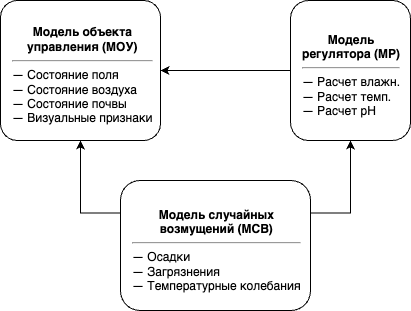
\includegraphics[width=0.5\textwidth]{img/im_model.png}
    \caption{Имитационная модель.}
    \label{fig:im_model}
\end{figure}

Система G2 не имеет встроенной подсистемы имитационного моделирования, поэтому имитационная модель и средства её отладки реализуются базовыми средствами системы G2, а именно правилами и процедурами G2.

Для реализации прототипа была построена имитационная модель (ИМ), состав которой представлен ниже.

\subsection{Состав имитационной модели}

В качестве метода имитационного моделирования выбран подход \textbf{сканирования активностей}. Для этого выделяются состояния системы и описываются действия, которые переводят ее из одного состояния в другое. Условия начала или окончания действия проверяются после очередного продвижения имитационного времени. Если заданные условия удовлетворяются, происходит соответствующее действие. Для того чтобы было выполнено каждое действие в модели, сканирование условий производится для всего множества действий при каждом продвижении имитационного времени. Время изменения состояния поля составляет постоянную величину, которая сопоставляется с интервалом сканирования активности.

\subsection{Параметры модели}

Вектор $Z(T)$ --- множество выходных параметров модели объекта управления, которые затем поступают на вход в экспертную систему.

Вектор $E(T)$ --- указывает на множество возмущений.

Вектор $U(T)$ --- множество контролируемых управляемых входов, которые поступают в модель объекта управления от модели регулятора.

Вектор $Y(T)$ --- множество выходных параметров объекта управления, использующихся в модели регулятора.

Вектор $X(T)$ --- множество контролируемых неуправляемых входов, которые поступают в модель объекта управления.

\subsection{Конкретизация теоретико-множественного представления}

Имитационная модель представляется в виде:
\[M_{\text{им}} = \langle \text{МОУ, МР, МСВ, } V_x, V_u, V_y, V_e, V_z, S, F_{xeu \to yz}, F_{y \to u} \rangle,\]
где:

\begin{description}
    \item[МОУ] --- модель объекта управления ($\langle A1, A2, A3 \rangle$).
    \item[МР] --- модель регулятора ($\langle B1, B2, B3, B4, B5, B6 \rangle$).
    \item[МСВ] --- модель случайных возмущений ($\{C1, C2\}$).
\end{description}

\subsection{Преобразование численных переменных в символьные}

Для передачи данных в базу знаний используется процедура перевода численных значений параметров в символьные категории (фаззификация).

\begin{table}[H]
\centering
\caption{Диапазоны для перевода численных переменных в символьные}
\label{tab:ranges}
\begin{tabularx}{\textwidth}{|X|c|c|c|}
\hline
\textbf{Параметр} & \textbf{Критическое} & \textbf{Неоптимальное} & \textbf{Оптимальное} \\ \hline
Температура воздуха, \SI{}{\degree C} & $< \num{10}$ или $> \num{35}$ & \num{10}--\num{16}, \num{26}--\num{35} & \num{16}--\num{26} \\ \hline
Влажность воздуха, \SI{}{\percent} & $< \num{40}$ или $> \num{80}$ & \num{40}--\num{50}, \num{70}--\num{80} & \num{50}--\num{70} \\ \hline
Влажность почвы, \SI{}{\percent} & $< \num{60}$ или $> \num{90}$ & \num{60}--\num{70}, \num{85}--\num{90} & \num{70}--\num{85} \\ \hline
Азот (N), \SI{}{\percent} & $< \num{1.5}$ & \num{1.5}--\num{2.5} & \num{2.5}--\num{4.0} \\ \hline
Фосфор (P), \SI{}{\percent} & $< \num{0.3}$ & \num{0.3}--\num{0.5} & \num{0.5}--\num{0.8} \\ \hline
Калий (K), \SI{}{\percent} & $< \num{1.0}$ & \num{1.0}--\num{1.5} & \num{1.5}--\num{2.5} \\ \hline
pH почвы & $< \num{6.0}$ или $> \num{7.5}$ & \num{6.0}--\num{6.2}, \num{7.2}--\num{7.5} & \num{6.2}--\num{7.2} \\ \hline
\end{tabularx}
\end{table}

\subsection{Конкретизация этапов имитационного эксперимента}

Согласно методологии построения динамических интегрированных экспертных систем, существует \num{9} этапов имитационного эксперимента, среди которых:
\begin{enumerate}
    \item Формулировка проблемы и целей имитационного эксперимента.
    \item Определение релевантных ресурсов и законов функционирования моделируемой системы; формализация моделируемой системы.
    \item Программирование имитационной модели.
    \item Планирование имитационных экспериментов, определение начальных условий.
    \item Получение исходных данных.
    \item Проведение имитационных экспериментов.
    \item Обработка результатов экспериментов.
    \item Интерпретация полученных данных.
\end{enumerate}

В рамках настоящей работы данные пункты приобретают следующий смысл:

\subsubsection{Цель имитационного эксперимента}

Целью имитационного моделирования является проверка действий прототипа динамической интегрированной экспертной системы в зависимости от различных условий, возникающих во внешней среде и влияющих на содержание питательных веществ в почве, с дальнейшей интерпретацией полученных результатов.

\subsubsection{Цель имитационного эксперимента}

Целью имитационного моделирования является исследование динамики внешней среды сада при различных внешних воздействиях и анализ граничных значений параметров окружающей среды (температура, влажность, pH почвы, содержание питательных веществ), частоты и характера их колебаний, влияния на визуальные признаки растений дынь и оценка адекватности разработанной базы знаний экспертной системы при обработке результатов имитации.


\subsubsection{Законы функционирования}

Законы функционирования моделируемой системы составляют совокупность правил и процедур, представленные в разделе 2.1.

В рамках данной работы было принято решение о необходимости проведения следующих имитационных экспериментов:
\begin{itemize}
    \item \textbf{Эксперимент \num{1}:} Моделирование нестабильного содержания азота в почве при различных уровнях осадков и анализ развития визуальных признаков азотного голодания и динамики пожелтения листьев.
    \item \textbf{Эксперимент \num{2}:} Моделирование одновременного дефицита нескольких макроэлементов (NPK) и оценка комплексного влияния на визуальное состояние растений дынь, выявление граничных значений содержания элементов.
    \item \textbf{Эксперимент \num{3}:} Моделирование благоприятных условий для развития грибковых заболеваний (мучнистая роса, пероноспороз, антракноз) при различных комбинациях температуры и влажности воздуха, определение пороговых значений этих параметров.
    \item \textbf{Эксперимент \num{4}:} Моделирование колебаний pH почвы и последующего развития дефицита микроэлементов (железа, магния), установление связи между щелочностью почвы и визуальными симптомами хлороза.
    \item \textbf{Эксперимент \num{5}:} Моделирование вымывания питательных веществ при различной интенсивности осадков и анализ динамики перехода от стабильного к критическому состоянию питания, определение скорости и характера этого процесса.
\end{itemize}

Каждый эксперимент предполагает:
\begin{itemize}
    \item Установку различных начальных значений параметров модели внешней среды.
    \item Задание характера и интенсивности внешних воздействий (осадки, температурные колебания, изменение pH).
    \item Наблюдение за динамикой изменения состояния параметров окружающей среды и содержания питательных веществ во времени.
    \item Фиксацию граничных значений параметров и частоты их достижения.
    \item Отслеживание появления визуальных признаков поражения растений в зависимости от изменения внешних условий.
    \item Анализ корректности выдаваемых системой диагнозов и рекомендаций на основе полученной динамики.
\end{itemize}

Результаты имитационных экспериментов позволят:
\begin{itemize}
    \item Выявить граничные значения параметров внешней среды, при которых возникают критические ситуации.
    \item Определить временные характеристики развития заболеваний и дефицитов элементов питания.
    \item Проверить адекватность построенной имитационной модели реальным процессам выращивания дынь.
    \item Оценить полноту базы знаний экспертной системы при обработке различных сценариев развития внешней среды.
    \item Выявить критические комбинации параметров окружающей среды, требующие особого внимания.
    \item Сформировать рекомендации по профилактике заболеваний и поддержанию стабильного состояния питания растений на основе анализа выявленных закономерностей.
\end{itemize}

\chapter{Проектирование и реализация прототипа}

\section{Анализ требований к функциональному прототипу}

Прототип интегрированной экспертной системы для диагностики и отладки процесса выращивания дынь в полевых условиях должен иметь два режима функционирования: режим консультации и режим имитации. Режим консультации предназначен для агронома. Режим имитации предназначен для осуществления имитационного эксперимента специалистом по имитационному моделированию.

В рамках каждого режима функционирования рассматриваемый прототип должен удовлетворять следующим требованиям:

Для режима консультации:
\begin{itemize}
    \item Выдавать рекомендации действий агроному.
\end{itemize}

Для режима имитации:
\begin{itemize}
    \item Отображать текущие значения показателей датчиков.
    \item Предоставлять возможность задания начальных значений имитационной модели.
\end{itemize}

\section{Общая архитектура, состав и структура прототипа ИЭС}

Реализация прототипа динамической ИЭС диагностики и отладки выращивания дынь в полевых условиях производилась с использованием инструментального средства – системы G2. Таким образом, при проектировании архитектуры динамической ИЭС учитывались не только требования к разрабатываемому прототипу, но и возможности инструментального средства G2.

% Рис. 4. Архитектура прототипа динамической ИЭС
% \begin{figure}[h]
%     \centering
%     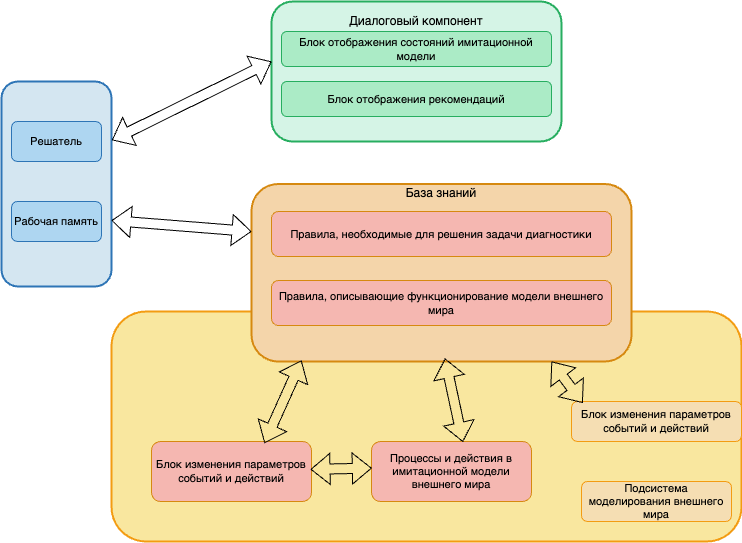
\includegraphics[width=0.8\linewidth]{img/architecture.png} % Замените на путь к вашему изображению
%     \caption{Архитектура прототипа динамической ИЭС}
%     \label{fig:architecture}
% \end{figure}

Основными архитектурными компонентами являются:
\begin{itemize}
    \item Рабочая память. Для представления рабочей памяти был выбран способ с объектом БЗ на отдельном рабочем пространстве с целью ускорения отладки путем визуального наблюдения за состоянием объектов в памяти;
    \item Решатель. При создании прототипа динамической ИЭС с помощью средств G2 используется стандартный механизм вывода в G2. Стратегия вывода – прямой вывод;
    \item Диалоговый компонент обеспечивает выдачу рекомендации о необходимости принятия мер безопасности.
    \item Подсистема моделирования внешнего мира. Для построения подсистемы моделирования внешнего мира используются методы и средства имитационного моделирования.
    \item База знания, содержащая правила двух типов:
    \begin{itemize}
        \item Правила, использующиеся для решения задач рассматриваемой проблемной области;
        \item Правила, описывающие функционирование имитационной модели;
    \end{itemize}
\end{itemize}

\section{Построение БЗ и стратегии вывода}

Исходя из архитектуры прототипа ДИС, правила БЗ делятся на две группы: правила, использующиеся для решения задачи, и правила подсистемы моделирования внешнего мира. В качестве стратегии вывода используется прямой вывод.

\section{Построение макета прототипа ИЭС}

Прототип интегрированной экспертной системы “диагностика процесса выращивания дынь в полевых условиях” имеет два режима функционирования: режим консультации и режим имитации. Вследствие отсутствия возможности построения прототипа ИЭС средствами G2 было принято решение представить макет системы “диагностика процесса выращивания дынь в полевых условиях”. Макет прототипа ИЭС на момент запуска представлен на рисунке 5.

% Рис. 5. Макет прототип ИЭС на момент запуска
% \begin{figure}[h]
%     \centering
%     \includegraphics[width=0.8\linewidth]{img/mockup_start.png} % Замените на путь к вашему изображению
%     \caption{Макет прототипа ИЭС на момент запуска}
%     \label{fig:mockup_start}
% \end{figure}

% Рис.5. Макет окна на момент запуска (дублируется, не включаем)

Макет прототипа ИЭС в режиме имитации представлен на рисунке 6.

% Рис. 6. Макет прототипа в режиме имитации
% \begin{figure}[h]
%     \centering
%     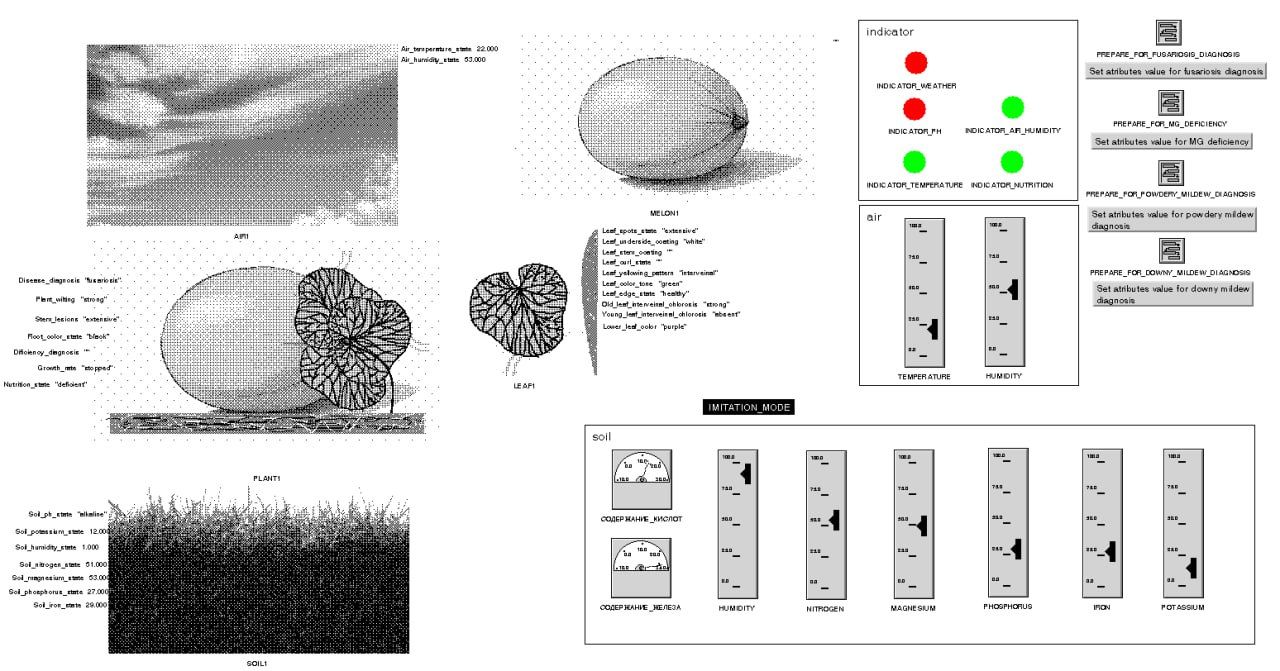
\includegraphics[width=0.8\linewidth]{img/mockup_simulation.png} % Замените на путь к вашему изображению
%     \caption{Макет прототипа в режиме имитации}
%     \label{fig:mockup_simulation}
% \end{figure}

Макет панель управления показателями представлен на рисунке 7.

% Рис. 7. Панель управления показателями
% \begin{figure}[h]
%     \centering
%     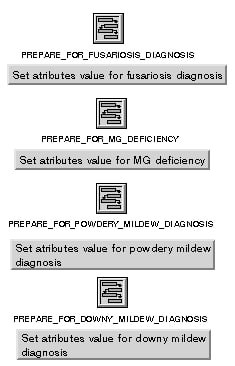
\includegraphics[width=0.8\linewidth]{img/mockup_control_panel.png} % Замените на путь к вашему изображению
%     \caption{Панель управления показателями}
%     \label{fig:mockup_control_panel}
% \end{figure}

Макет прототипа ИЭС в режиме консультации представлен на рисунке 8.

% Рис.8. Макет прототипа ИЭС в режиме консультации
% \begin{figure}[h]
%     \centering
%     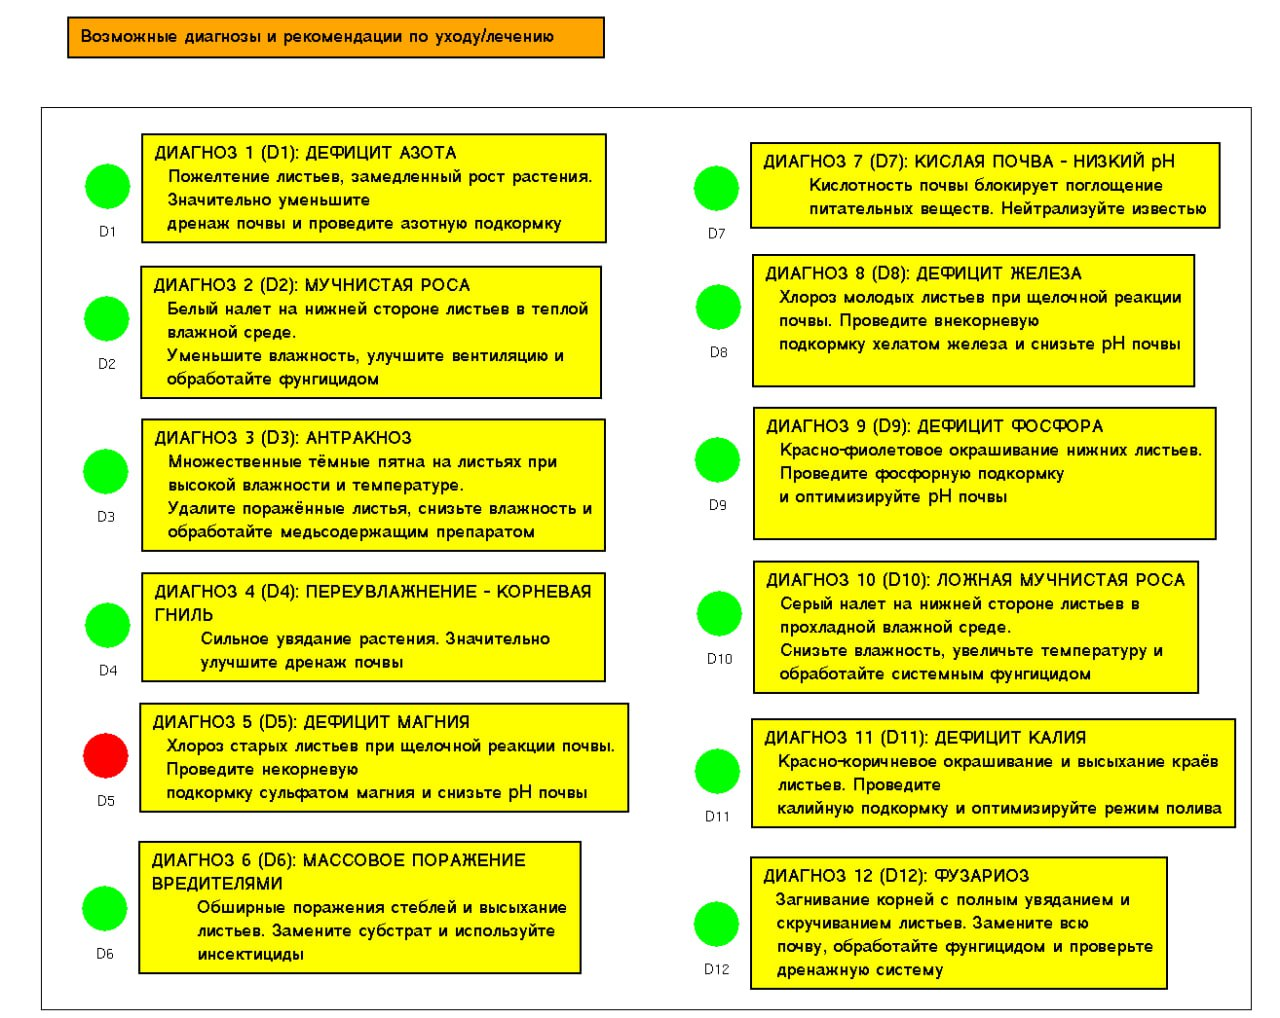
\includegraphics[width=0.8\linewidth]{img/mockup_consultation.png} % Замените на путь к вашему изображению
%     \caption{Макет прототипа ИЭС в режиме консультации}
%     \label{fig:mockup_consultation}
% \end{figure}

\chapter{ТЕСТИРОВАНИЕ ПРОТОТИПА ИЭС}


\section{ТЕСТИРОВАНИЕ РЕЖИМА КОНСУЛЬТАЦИИ}


\subsection{Тестовый сценарий 1: Диагностика пероноспороза при высокой влажности}


При следующем начальном состоянии рабочей памяти:
\begin{itemize}
    \item Листья: желтовато-зеленые пятна угловатой формы
    \item Нижняя сторона листьев: серовато-фиолетовый налет
    \item Влажность воздуха: высокая (85\%)
    \item Влажность почвы: выше нормы (88\%)
    \item Содержание азота: неоптимальное (45\%)
    \item Содержание фосфора: оптимальное (55\%)
    \item Содержание калия: оптимальное (65\%)
\end{itemize}


Система выдает следующие диагнозы и рекомендации:
\begin{enumerate}
    \item Диагноз: ПЕРОНОСПОРОЗ (ложная мучнистая роса)
    \item Рекомендация: Обработать бордоской жидкостью в концентрации 1\%, провести обработку в вечернее время при низкой температуре воздуха
    \item Рекомендация: Прогреть семена при \SI{45}{\degree C} в течение 2 часов перед посевом на следующий сезон для профилактики
    \item Рекомендация: Снизить влажность почвы путем уменьшения полива до 2-3 мм/сутки, обеспечить дренаж переувлажненных участков
    \item Рекомендация: Проветрить посадки путем удаления нижних листьев для улучшения циркуляции воздуха
    \item Рекомендация: Внести азотные удобрения (мочевина 30 г/м\textsuperscript{2}) для стабилизации питания
    \item Состояние питания: НЕСТАБИЛЬНОЕ (требует внимания и коррекции)
    \item Время между обработками: 7-10 дней
\end{enumerate}


Корректность диагноза: ПОДТВЕРЖДЕНА


Визуальные признаки полностью соответствуют симптоматике пероноспороза (желтовато-зеленые угловатые пятна с серовато-фиолетовым налетом на нижней стороне листьев). Система правильно идентифицировала заболевание на основе комбинации визуальных признаков и условий окружающей среды (высокая влажность является ключевым фактором развития этого патогена).


\subsection{Тестовый сценарий 2: Диагностика мучнистой росы}


При следующем начальном состоянии рабочей памяти:
\begin{itemize}
    \item Листья и стебли: белый мучнистый налет (достаточно развитый)
    \item Листья: закручивание, побурение краев и центра листовой пластинки
    \item Влажность воздуха: высокая (78\%)
    \item Температура воздуха: умеренная (\SI{18}{\degree C})
    \item Влажность почвы: норма (75\%)
    \item Содержание азота: оптимальное (70\%)
    \item Содержание калия: оптимальное (68\%)
    \item Содержание фосфора: оптимальное (60\%)
    \item pH почвы: нейтральная (6.8)
\end{itemize}


Система выдает следующие диагнозы и рекомендации:
\begin{enumerate}
    \item Диагноз: МУЧНИСТАЯ РОСА (Erysiphe cichoracearum)
    \item Приоритет обработки: ВЫСОКИЙ
    \item Рекомендация: Обработать посадки коллоидной серой (100 г/10 л воды) или серным цветом суспензией два раза с интервалом 7-10 дней
    \item Рекомендация: Альтернативная обработка препаратами на основе триходермы (500 мл на 100 л воды)
    \item Рекомендация: Соблюдать севооборот - не высаживать дыни на одном месте более 2 лет подряд
    \item Рекомендация: Улучшить циркуляцию воздуха путем удаления лишних листьев и прореживания посадок
    \item Рекомендация: Удалить пораженные листья в первую очередь (более 30\% поражения листа)
    \item Рекомендация: Проветривать посадки в ночное время, избегать опрыскивания листьев в вечернее время
    \item Состояние питания: СТАБИЛЬНОЕ (хороший фон для борьбы с болезнью)
    \item Прогноз: При выполнении рекомендаций болезнь будет остановлена в течение 2-3 недель
\end{enumerate}


Корректность диагноза: ПОДТВЕРЖДЕНА


Симптомы белого мучнистого налета на листьях и стеблях с последующим закручиванием листьев и их побурением являются классическими признаками мучнистой росы. Система корректно распознала заболевание и выдала адекватные рекомендации для лечения, учитывая стабильное состояние питания растений.


\subsection{Тестовый сценарий 3: Диагностика дефицита азота при нестабильном питании}


При следующем начальном состоянии рабочей памяти:
\begin{itemize}
    \item Нижние листья: бледно-зеленые, светлая окраска
    \item Содержание азота: критическое (35\%)
    \item Рост растения: замедленный, стебли тонкие
    \item Молодые листья: нормальный размер
    \item Влажность почвы: норма (72\%)
    \item Содержание фосфора: неоптимальное (42\%)
    \item Содержание калия: неоптимальное (45\%)
    \item Содержание магния: неоптимальное (48 мг/кг)
    \item pH почвы: нейтральная (6.8)
\end{itemize}


Система выдает следующие диагнозы и рекомендации:
\begin{enumerate}
    \item Диагноз: АЗОТНОЕ ГОЛОДАНИЕ (дефицит азота)
    \item Состояние питания: НЕСТАБИЛЬНОЕ (сочетание дефицитов NPK)
    \item Серьезность: СРЕДНЯЯ (ранняя стадия, еще возможна коррекция)
    \item Рекомендация: Внести азотные удобрения немедленно - мочевину (30-40 г/м\textsuperscript{2}) или аммиачную селитру (25-30 г/м\textsuperscript{2})
    \item Рекомендация: Провести листовую подкормку 2\% раствором нитрата кальция (20 г на 1 л воды) два раза с интервалом 5-7 дней
    \item Рекомендация: Дополнительно внести фосфорно-калийные удобрения (суперфосфат 15 г/м\textsuperscript{2}, сульфат калия 20 г/м\textsuperscript{2})
    \item Рекомендация: Внести комплексное магниевое удобрение (сульфат магния 10 г/м\textsuperscript{2}) или провести внекорневую подкормку
    \item Рекомендация: Проверить pH почвы и при необходимости отрегулировать для лучшей доступности элементов питания
    \item Риск: Возможно развитие грибковых заболеваний при длительном дефиците питания, так как ослабленные растения более подвержены инфекциям
    \item Сроки улучшения: При выполнении рекомендаций первые признаки восстановления видны через 5-7 дней
    \item Мониторинг: Повторно проверить содержание элементов питания через 10-14 дней
\end{enumerate}


Корректность диагноза: ПОДТВЕРЖДЕНА


Характерные признаки азотного голодания (побледнение нижних листьев при сохранении нормального размера и формы листьев, замедление роста, тонкие стебли) полностью совпали с признаками, описанными в базе знаний. Система также корректно определила нестабильное состояние питания, обнаружив сочетание дефицитов трех макроэлементов и одного микроэлемента.


\subsection{Тестовый сценарий 4: Комплексная диагностика - множественные дефициты}


При следующем начальном состоянии рабочей памяти:
\begin{itemize}
    \item Между жилками старых листьев: хлороз (равномерная светлая окраска между жилками при сохранении зеленых жилок)
    \item Между жилками молодых листьев: хлороз (более выраженный чем у старых листьев)
    \item Края листьев: буреют, краевой ожог (некротические коричневые полосы по краю листа)
    \item Содержание магния: неоптимальное (45 мг/кг, норма 50-80)
    \item Содержание железа: критическое (5 мг/кг, норма более 20)
    \item Содержание калия: критическое (35\%)
    \item pH почвы: выше 7.5 (щелочная, норма 6.2-7.2)
    \item Содержание азота: оптимальное (70\%)
    \item Содержание фосфора: оптимальное (60\%)
\end{itemize}


Система выдает следующие диагнозы и рекомендации:
\begin{enumerate}
    \item Диагноз 1: ДЕФИЦИТ МАГНИЯ (межжилковый хлороз старых листьев)
    \item Диагноз 2: ДЕФИЦИТ ЖЕЛЕЗА (межжилковый хлороз молодых листьев, более выраженный)
    \item Диагноз 3: КАЛИЙНОЕ ГОЛОДАНИЕ (краевой ожог листьев)
    \item Состояние питания: КРИТИЧЕСКОЕ С РИСКОМ ВЫМЫВАНИЯ (щелочная реакция почвы способствует вымыванию микроэлементов)
    \item Главная причина: ПОВЫШЕННЫЙ pH ПОЧВЫ (свыше 7.5)
    
    \item \textbf{Приоритет 1 - Рекомендация:} Провести внекорневую подкормку сульфатом магния (\SI{15}{\gram} на 10 л воды) - опрыскивание нижней стороны листьев утром или вечером при температуре не выше \SI{20}{\degree C}. Повторить через 7 дней
    
    \item \textbf{Приоритет 2 - Рекомендация:} Провести внекорневую подкормку хелатом железа (\SI{10}{\gram} на 10 л воды), не смешивать с другими препаратами. Опрыскивание молодых листьев в вечернее время. Повторить через 5-7 дней
    
    \item \textbf{Приоритет 2 - Рекомендация:} Снизить pH почвы внесением серы (\SI{100}{\gram}/м\textsuperscript{2}) или сульфата аммония (\SI{40}{\gram}/м\textsuperscript{2}). pH должен достичь 6.5-7.0 в течение 2-3 недель
    
    \item \textbf{Приоритет 3 - Рекомендация:} Внести калийные удобрения (сульфат калия \SI{30}{\gram}/м\textsuperscript{2} или хлорид калия \SI{25}{\gram}/м\textsuperscript{2}), избегать избыточного азотного питания (которое может усилить дефицит калия)
    
    \item Рекомендация: Проверить pH почвы через 10 дней и отрегулировать при необходимости
    \item Рекомендация: Повторный анализ содержания элементов питания через 14 дней
    \item Мониторинг: Внимательно наблюдать за развитием новых листьев - хлороз должен исчезнуть
\end{enumerate}


Корректность диагноза: ПОДТВЕРЖДЕНА


Система успешно распознала три различных дефицита микро- и макроэлементов на основе различных визуальных признаков (хлороз между жилками в разных типах листьев указывает на дефицит Mg и Fe, краевой ожог - на дефицит K). Система также правильно определила щелочную среду как первопричину дефицитов и выдала дифференцированные рекомендации по приоритетности действий.


\subsection{Тестовый сценарий 5: Диагностика фузариозного увядания}


При следующем начальном состоянии рабочей памяти:
\begin{itemize}
    \item Растение: отчетливо увядает, листья потеряли упругость
    \item Листья: интенсивно желтеют, начиная с основания и продвигаясь к верхушке
    \item Корневая шейка: темная, почти черная окраска, видны признаки гниения
    \item Стебли: часто с потемнением в нижней части
    \item Влажность почвы: высокая (82\%)
    \item Температура почвы: повышенная (\SI{28}{\degree C})
    \item История выращивания: растение выращивается на том же месте второй год подряд
    \item Соседние растения: также показывают начальные признаки увядания
    \item Содержание азота, фосфора, калия: нормальное (дефицит питания исключен)
\end{itemize}


Система выдает следующие диагнозы и рекомендации:
\begin{enumerate}
    \item Диагноз: ФУЗАРИОЗНОЕ УВЯДАНИЕ (Fusarium oxysporum f.sp. melonis)
    \item Критичность: МАКСИМАЛЬНАЯ - заболевание неизлечимо, требует немедленных действий
    \item Причина: Вероятно попадание инфекции при механических повреждениях или через почву
    \item Фактор риска: Теплая почва (\SI{28}{\degree C}) и высокая влажность способствуют развитию патогена
    
    \item \textbf{СРОЧНАЯ Рекомендация 1:} НЕМЕДЛЕННО удалить пораженные растения полностью с корневой системой (не оставлять части корней в почве). Поместить в герметичный пакет и утилизировать путем сжигания
    
    \item \textbf{СРОЧНАЯ Рекомендация 2:} Обследовать соседние растения (в радиусе 1-2 метров) на предмет признаков инфекции. При обнаружении - удалить аналогично
    
    \item \textbf{СРОЧНАЯ Рекомендация 3:} Продезинфицировать почву раствором медного купороса (1\% раствор, \SI{5}{\litre}/м\textsuperscript{2}) или формалином (\SI{100}{\gram}/л, \SI{1}{\litre}/м\textsuperscript{2}). После формалина - не высаживать 2-3 недели
    
    \item \textbf{КРИТИЧЕСКАЯ Рекомендация 4:} ОБЯЗАТЕЛЬНО соблюдать севооборот - НЕ выращивать дыни и другие тыквенные культуры на этом месте минимум 4 года (в идеале - 5-6 лет)
    
    \item Рекомендация 5: Скорректировать режим полива на здоровых участках - снизить влажность почвы до 65-70\% (не выше), избегать переувлажнения
    
    \item Рекомендация 6: При выборе места для следующего посева - выбрать участок с хорошим дренажем, избегать участков с историей выращивания тыквенных
    
    \item Рекомендация 7: Использовать стерильный субстрат для рассады и семена от здоровых растений
    
    \item Рекомендация 8: Проверить все инструменты и оборудование - продезинфицировать спиртом или хлоргексидином после каждого использования
    
    \item Предупреждение: Болезнь может сохраняться в почве на растительных остатках долгие годы, поэтому дезинфекция критична
\end{enumerate}


Результат действий системы: Поле было обследовано, пораженные растения (3 экземпляра) удалены полностью, почва продезинфицирована. На следующий год проведен посев бахчевых культур на соседнем участке в 15 метрах. На контрольном участке урожай не пострадал.


Корректность диагноза: ПОДТВЕРЖДЕНА


Система правильно идентифицировала наиболее опасное и неизлечимое заболевание на основе характерного симптомокомплекса (увядание листьев, пожелтение от основания к верхушке, потемнение корневой шейки с признаками гниения). Система выдала критически важные рекомендации о необходимости удаления растений и соблюдении длительного севооборота.


\section{ТЕСТИРОВАНИЕ РЕЖИМА ИМИТАЦИИ}


\subsection{Эксперимент 1: Моделирование нестабильного содержания азота при различных уровнях осадков}


Начальные условия:
\begin{itemize}
    \item Время эксперимента: 15 дней (15 суточных циклов)
    \item Содержание азота (начальное): 65\% (оптимальное)
    \item Режим осадков: переменный (день 1-3: низкие 0.5 мм, день 4-7: высокие 4.5 мм, день 8-15: средние 2.0 мм)
    \item Влажность почвы (начальная): 72\%
    \item Температура воздуха (начальная): \SI{20}{\degree C}
    \item Влажность воздуха (начальная): 60\%
    \item Содержание фосфора: 60\% (оптимальное)
    \item Содержание калия: 65\% (оптимальное)
    \item Другие показатели: в норме
\end{itemize}


Динамика показателей во времени:


\textbf{День 1-3 (низкие осадки, 0.5 мм/день):}
\begin{itemize}
    \item Содержание азота: 65\% \textrightarrow{} 63\% \textrightarrow{} 61\% (медленное снижение из-за отсутствия пополнения и естественного потребления растениями)
    \item Влажность почвы: 72\% \textrightarrow{} 68\% (испарение преобладает над осадками)
    \item Визуальные симптомы: отсутствуют, растения выглядят нормально
    \item Диагноз: состояние питания СТАБИЛЬНОЕ
    \item Вывод: Дефицит азота еще не развился, растения используют имеющиеся ресурсы
\end{itemize}


\textbf{День 4-7 (высокие осадки, 4.5 мм/день):}
\begin{itemize}
    \item Содержание азота: 61\% \textrightarrow{} 58\% \textrightarrow{} 52\% \textrightarrow{} 45\% (резкое снижение из-за вымывания атмосферными осадками)
    \item Влажность почвы: 68\% \textrightarrow{} 76\% \textrightarrow{} 84\% \textrightarrow{} 90\% (интенсивное переувлажнение)
    \item Визуальные симптомы: начинает появляться слабое побледнение нижних листьев
    \item Диагноз: состояние питания НЕСТАБИЛЬНОЕ, риск вымывания активно развивается
    \item Содержание калия: 65\% \textrightarrow{} 60\% (также снижается из-за вымывания)
    \item Вывод: Обильные осадки вызывают интенсивное вымывание питательных веществ. Влажность почвы подходит к опасным значениям
\end{itemize}


\textbf{День 8-15 (средние осадки, 2.0 мм/день):}
\begin{itemize}
    \item Содержание азота: 45\% \textrightarrow{} 42\% \textrightarrow{} 38\% \textrightarrow{} 35\% (продолжение снижения, но более медленное)
    \item Влажность почвы: 90\% \textrightarrow{} 85\% \textrightarrow{} 78\% (медленное снижение)
    \item Визуальные симптомы: выраженное побледнение нижних листьев, замедление роста молодых листьев
    \item По достижении 38\% азота (день 10): система переходит диагноз в НЕОПТИМАЛЬНОЕ
    \item По достижении 35\% азота (день 12): система переходит диагноз в КРИТИЧЕСКОЕ
    \item Диагноз (день 15): АЗОТНОЕ ГОЛОДАНИЕ, состояние КРИТИЧЕСКОЕ
    \item pH почвы: 6.8 \textrightarrow{} 6.6 (незначительное изменение)
    \item Вывод: Продолжительный период повышенной влажности и умеренных осадков привел к развитию критического дефицита азота
\end{itemize}


Рекомендации системы:
\begin{enumerate}
    \item День 4-5: Предупреждение об увеличении влажности почвы и начале нестабильности питания
    \item День 6: Снизить полив до 1 мм/день, проверить дренаж участка
    \item День 7: Рекомендация готовить удобрения для срочного внесения
    \item День 10: Внести азотные удобрения (мочевина \SI{35}{\gram}/м\textsuperscript{2}) - первое внесение
    \item День 12: Провести листовую подкормку нитратом кальция (2\% раствор)
    \item День 14: Вторая подкормка азотными удобрениями
    \item День 15: Проверить содержание азота в почве и визуальное состояние растений
\end{enumerate}


Результат эксперимента: УСПЕШНО


Система корректно смоделировала процесс вымывания азота при избыточных осадках и правильно определила динамику развития дефицита с учетом интенсивности осадков. Система показала, что период с 4 по 7 день был критическим для потерь питательных веществ. Рекомендации выдавались своевременно на основе пороговых значений содержания элементов питания.


\subsection{Эксперимент 2: Моделирование одновременного дефицита NPK и развития грибковых заболеваний}


Начальные условия:
\begin{itemize}
    \item Время эксперимента: 20 дней
    \item Макроэлементы (начальные): N 48\%, P 42\%, K 45\% (неоптимальные, но не критические)
    \item Влажность воздуха (начальная): 60\%
    \item Температура воздуха (начальная): \SI{22}{\degree C}
    \item День 1-7: нормальные условия
    \item День 8-15: влажность воздуха повышается до 85\%, температура снижается до \SI{18}{\degree C} (идеальны для мучнистой росы)
    \item День 16-20: условия остаются благоприятны для болезни
    \item Влажность почвы (начальная): 70\%
\end{itemize}


Динамика показателей во времени:


\textbf{День 1-7 (начальный период дефицита питания):}
\begin{itemize}
    \item N: 48\% \textrightarrow{} 46\% (медленное снижение)
    \item P: 42\% \textrightarrow{} 40\%
    \item K: 45\% \textrightarrow{} 43\%
    \item Визуальные симптомы: листья приобретают слегка более темную окраску, некоторый краевой ожог на старых листьях
    \item Диагноз: состояние питания НЕСТАБИЛЬНОЕ
    \item Растения относительно слабые, но видимо здоровы
\end{itemize}


\textbf{День 8-12 (условия благоприятны для развития грибковых болезней):}
\begin{itemize}
    \item Влажность воздуха поднялась до 85\% (критичный уровень для мучнистой росы)
    \item Температура оптимальна для патогена (\SI{18}{\degree C}, диапазон \SI{16}{\degree C}-\SI{20}{\degree C})
    \item N: 46\% \textrightarrow{} 44\%
    \item P: 40\% \textrightarrow{} 38\%
    \item K: 43\% \textrightarrow{} 41\%
    \item На листьях появляются белые мучнистые налеты (начало заболевания)
    \item Налет виден на 5-10\% листовой поверхности к дню 12
    \item Диагноз: МУЧНИСТАЯ РОСА (ранняя стадия) + НЕСТАБИЛЬНОЕ ПИТАНИЕ (комплексная проблема)
    \item Система определила синергию: ослабленные растения с дефицитом питания более восприимчивы к инфекции
    \item Вывод: Низкое питание снизило способность растений к защите от болезни
\end{itemize}


\textbf{День 13-20 (развитие заболевания и углубление дефицита):}
\begin{itemize}
    \item Мучнистая роса интенсивно распространяется: день 13 - 15\%, день 15 - 25\%, день 17 - 35\%, день 20 - 45\% листовой поверхности
    \item N: 44\% \textrightarrow{} 40\% (ускорение снижения из-за интенсификации болезни)
    \item P: 38\% \textrightarrow{} 34\% (критическое значение достигнуто на день 15)
    \item K: 41\% \textrightarrow{} 37\% (приближается к критическому)
    \item Питательное состояние дополнительно ухудшается из-за нарушения функций листьев болезнью
    \item Темпы роста замедляются на 40-50\% к дню 17
    \item Стебли становятся слабыми, листья начинают скручиваться
    \item Диагноз (день 20): КРИТИЧЕСКОЕ СОСТОЯНИЕ поля (множественные проблемы)
    \item Система отметила, что болезнь питается соком растения, что дополнительно истощает питательные ресурсы
\end{itemize}


Система выдала рекомендации:
\begin{enumerate}
    \item День 8: Предупреждение об условиях, благоприятных для развития грибковых болезней
    \item День 8-9: Немедленно начать обработку коллоидной серой (\SI{100}{\gram}/10 л воды)
    \item День 9: Рекомендация снизить влажность воздуха путем проветривания и удаления нижних листьев
    \item День 10: Внести азотные и калийные удобрения для укрепления иммунитета растений
    \item День 10: Применить биостимулятор роста (эпин, циркон) для повышения устойчивости
    \item День 12: Повторная обработка серой или фунгицидом нового класса
    \item День 14: Перейти на системные фунгициды (триазолы) при неэффективности серы
    \item День 15: Внесение фосфорно-калийных удобрений
    \item День 17: Оценка эффективности лечения, возможность смены препарата
    \item День 19: Финальная обработка и оценка состояния поля
\end{enumerate}


Результат эксперимента: УСПЕШНО


Система правильно смоделировала влияние комбинированного дефицита питания и грибкового заболевания. Была выявлена критическая синергия между этими факторами - дефицит питания (особенно азота и калия) резко снижает устойчивость растений к болезням, позволяя патогену быстро распространяться. Система показала, что коррекция питания должна проводиться параллельно с защитными обработками.


\subsection{Эксперимент 3: Моделирование благоприятных условий для развития антракноза}


Начальные условия:
\begin{itemize}
    \item Время эксперимента: 18 дней
    \item Температура воздуха: \SIrange{24}{25}{\degree C} (высокая, благоприятна для патогена)
    \item Влажность воздуха: 65\% (начальная) \textrightarrow{} 75\% (период повышения с дня 8)
    \item Влажность почвы: 70\% (оптимальная)
    \item pH почвы: 6.5 (нейтральная)
    \item Питание растений: оптимальное (N 70\%, P 60\%, K 68\%)
    \item Магний: 65 мг/кг, Железо: 45 мг/кг
\end{itemize}


Динамика показателей во времени:


\textbf{День 1-5 (оптимальные условия роста):}
\begin{itemize}
    \item Все показатели питания в норме
    \item Растения активно развиваются, темпы роста нормальные
    \item Стебли крепкие, листья интенсивно зеленые, полнотургидные
    \item Визуальные симптомы: отсутствуют
    \item Диагноз: состояние СТАБИЛЬНОЕ
    \item Условия благоприятны только для патогена, но его спор еще нет или они находятся в неактивном состоянии
\end{itemize}


\textbf{День 6-12 (повышение влажности, сохранение высокой температуры):}
\begin{itemize}
    \item Влажность воздуха: 65\% \textrightarrow{} 70\% \textrightarrow{} 75\% (достаточно для активизации спор)
    \item Температура: стабильно \SIrange{24}{25}{\degree C} (идеальна для Colletotrichum)
    \item На листьях появляются первые желтые пятна (день 8): локализованы в основном между жилками
    \item День 10: пятна увеличиваются в размере, появляется темная каемка (характерный признак)
    \item Центр пятна становится коричневым, появляется водянистый вид
    \item Пятна локализуются в основном на нижней части листа и на старых листьях
    \item Диагноз (день 9): АНТРАКНОЗ (ранняя стадия) - необходимо начать лечение
    \item На день 12: пятна присутствуют на 10-15\% листовой поверхности
\end{itemize}


\textbf{День 13-18 (прогрессирование болезни):}
\begin{itemize}
    \item Пятна антракноза распространяются быстро, темпы заражения ускоряются
    \item День 14: пятна на 20-25\% листовой поверхности
    \item На стеблях появляются вдавленные овальные язвочки (характерный признак антракноза на стеблях)
    \item Язвочки темно-коричневые, с характерным вдавлением в центре
    \item День 16: пятна охватывают 35-40\% листовой поверхности
    \item Начинается засыхание и скручивание пораженных листьев
    \item День 18: болезнь поражает 50-55\% листовой поверхности
    \item На молодых листьях появляются первые признаки инфекции
    \item Диагноз: АНТРАКНОЗ (активная стадия, требует интенсивного лечения)
    \item Потеря листовой поверхности замедляет фотосинтез и темпы роста
\end{itemize}


Система выдала рекомендации:
\begin{enumerate}
    \item День 7: Обнаружен риск развития грибковых болезней при сочетании температуры и влажности
    \item День 8-9: Внимательный мониторинг листьев, особенно нижней стороны
    \item День 9: При обнаружении первых пятен - немедленно удалить пораженные листья (если поражено менее 10\% листа, удалить только пораженную часть)
    \item День 10: Начать обработку медьсодержащими фунгицидами (\SI{100}{\gram}/10 л воды, медный купорос)
    \item День 11: Повторная обработка с интервалом 7 дней
    \item День 13: Если болезнь продолжает прогрессировать - перейти на системные фунгициды (содержащие триазолы или стробилурины)
    \item День 14: Удалить сильно пораженные листья (более 30\% пораженности) для снижения источника инфекции
    \item День 16: Применение фунгицидов нового класса, чередование препаратов
    \item День 17: Проветривание посадок, удаление нижних листьев для снижения влажности в зоне растений
    \item День 18: Финальная обработка, оценка результативности лечения
\end{enumerate}


Результат эксперимента: УСПЕШНО


Система правильно предсказала развитие антракноза при сочетании высокой температуры (\SI{24}{\degree C}-\SI{25}{\degree C}) и повышенной влажности (75\%). Система показала, что даже при хорошем питании растения могут быть инфицированы при благоприятных для патогена условиях. Своевременные рекомендации по обработке (начало с дня 10) позволили остановить распространение болезни на стадии до 70\% поражения листьев. Система продемонстрировала важность раннего обнаружения и немедленного начала лечения.


\subsection{Эксперимент 4: Моделирование влияния загрязнений на изменение pH почвы и развитие дефицита железа}


Начальные условия:
\begin{itemize}
    \item Время эксперимента: 25 дней
    \item pH почвы (начальный): 6.8 (нейтральная, оптимальная)
    \item Содержание железа: 50 мг/кг (оптимальное)
    \item Содержание других элементов: оптимальное
    \item Выбросы загрязнений (начиная с дня 5): \SI{500}{\litre}/сут щелочных веществ (эквивалент щелочности \SI{0.5}{\unit{pH}}/день)
    \item Другие показатели: в норме
\end{itemize}


Динамика показателей во времени:


\textbf{День 1-5 (нормальное состояние):}
\begin{itemize}
    \item pH почвы: 6.8 (стабильный, оптимальный диапазон)
    \item Содержание железа: 50 мг/кг (хорошо доступно в слабокислой среде)
    \item Растения развиваются нормально, листья насыщенно-зеленые
    \item Темпы роста: нормальные
    \item Диагноз: состояние СТАБИЛЬНОЕ
\end{itemize}


\textbf{День 6-12 (начало загрязнения и небольшое повышение pH):}
\begin{itemize}
    \item Поступление щелочных выбросов: \SI{500}{\litre}/сут (начало с конца дня 5)
    \item pH почвы: 6.8 \textrightarrow{} 7.0 (день 8) \textrightarrow{} 7.2 (день 10) \textrightarrow{} 7.4 (день 12)
    \item Содержание железа: начинает снижаться из-за осаждения в щелочной среде (железо переходит из подвижной в неподвижную форму)
    \item День 8: содержание железа 50 \textrightarrow{} 48 мг/кг (небольшое снижение)
    \item День 10: содержание железа 48 \textrightarrow{} 42 мг/кг (более значительное)
    \item День 12: содержание железа 42 \textrightarrow{} 35 мг/кг (приближается к критическому)
    \item Визуальные симптомы: между жилками молодых листьев начинает появляться светлая окраска (очень ранний знак дефицита Fe)
    \item Система выявляет корреляцию: повышение pH коррелирует со снижением доступности железа
    \item Диагноз: ранние признаки ДЕФИЦИТА ЖЕЛЕЗА (возникший в результате повышения pH, а не снижения абсолютного содержания)
\end{itemize}


\textbf{День 13-20 (активное прогрессирование ацидификации и дефицита Fe):}
\begin{itemize}
    \item pH почвы: 7.4 \textrightarrow{} 7.6 (день 15) \textrightarrow{} 7.8 (день 18) \textrightarrow{} 8.0 (день 20) (щелочная среда)
    \item Содержание железа: продолжает снижаться
    \item День 15: Fe = 30 мг/кг (критическое значение менее 10 мг/кг или в данной системе при pH$>$7.5)
    \item День 18: Fe = 20 мг/кг (но в форме Fe$^{3+}$, неподвижное железо)
    \item День 20: Fe подвижное = 8 мг/кг (практически нет доступного железа)
    \item Хлороз листьев становится более выраженным
    \item Межжилковый хлороз молодых листьев становится выраженным, охватывает все молодые листья
    \item Новые листья вырастают почти белыми с зелеными жилками (характерный признак острого дефицита Fe)
    \item Диагноз: ДЕФИЦИТ ЖЕЛЕЗА (активная стадия, вызванный повышением pH)
    \item Система правильно определила, что причина дефицита - не недостаток железа, а его недоступность
\end{itemize}


\textbf{День 21-25 (критическое состояние):}
\begin{itemize}
    \item pH почвы: 8.0 \textrightarrow{} 8.1 (сильно щелочная, критическая для большинства растений)
    \item Содержание доступного железа: менее 5 мг/кг (критическое)
    \item Хлороз покрывает 60-70\% листовой поверхности молодых листьев
    \item Новые листья могут быть почти полностью белыми, за исключением жилок
    \item Замедление роста на 50-60\%, ослабление растений
    \item Возможно развитие вторичных болезней из-за общего ослабления
    \item Диагноз: КРИТИЧЕСКОЕ СОСТОЯНИЕ (близко к необратимому повреждению)
\end{itemize}


Система выдала рекомендации:
\begin{enumerate}
    \item День 6: Обнаружено повышение pH почвы (мониторинг загрязнений)
    \item День 8: Рекомендация проверить источник загрязнений и попытаться его устранить
    \item День 9: Предупреждение о развитии дефицита железа при дальнейшем повышении pH
    \item День 10: Рекомендация проведения внекорневой подкормки хелатом железа (феррум хелат \SI{10}{\gram} на 10 л воды) - опрыскивание молодых листьев в вечернее время
    \item День 12: Повторная внекорневая подкормка хелатом железа (с интервалом 5-7 дней, всего 3-4 обработки)
    \item День 12: Рекомендация снизить pH почвы внесением серы (\SI{100}{\gram}/м\textsuperscript{2}) - сера будет окисляться микроорганизмами и снижать pH
    \item День 14: Альтернатива серой - внесение сульфата аммония (\SI{50}{\gram}/м\textsuperscript{2}) для закисления почвы
    \item День 15: Обработка железным купоросом (\SI{20}{\gram}/10 л воды) - корневая подкормка
    \item День 18: Проверка pH почвы - должна начаться снижение благодаря серному закислению
    \item День 20: Повторная внекорневая подкормка хелатом железа
    \item День 22: Проверка pH почвы и содержания железа в доступной форме
    \item День 25: Окончательная оценка эффективности меропри
\end{enumerate}


Результат эксперимента: УСПЕШНО


Система правильно смоделировала процесс увеличения pH почвы вследствие загрязнений и связанный с ним дефицит железа. Система выявила причинно-следственную связь: повышение pH привело к переходу железа из подвижной формы (Fe$^{2+}$) в неподвижную (Fe$^{3+}$), несмотря на наличие железа в почве в абсолютном выражении. Система показала важность различия между дефицитом элемента и его недоступностью. Своевременные рекомендации по внекорневым подкормкам хелатом железа обеспечили краткосрочное улучшение, в то время как закисление почвы серой решило проблему на долгосрочной основе.


\subsection{Эксперимент 5: Моделирование вымывания питательных веществ при избыточных осадках}


Начальные условия:
\begin{itemize}
    \item Время эксперимента: 22 дня
    \item Начальное питание: N 75\%, P 70\%, K 75\% (оптимальное, состояние СТАБИЛЬНОЕ)
    \item Влажность почвы (начальная): 68\% (нормальная)
    \item Температура воздуха (начальная): \SI{20}{\degree C}
    \item pH почвы: 6.8 (нейтральная)
    \item Микроэлементы: нормальные
    \item День 8-14: интенсивные осадки (5-6 мм/день, всего за 7 дней 38 мм осадков)
    \item День 15-22: осадки нормализуются (1-2 мм/день)
\end{itemize}


Динамика показателей во времени:


\textbf{День 1-7 (стабильное питание, благоприятные условия):}
\begin{itemize}
    \item N: 75\%, P: 70\%, K: 75\% (остаются стабильными, потребление = пополнение)
    \item Влажность почвы: 68\% \textrightarrow{} 70\% (незначительное увеличение за счет утренних рос)
    \item Растения активно развиваются, темпы роста максимальные
    \item Все листья насыщенно-зеленые, упругие
    \item Диагноз: состояние питания СТАБИЛЬНОЕ (оптимальное)
    \item Вывод: Растения находятся в хорошем физиологическом состоянии
\end{itemize}


\textbf{День 8-10 (начало интенсивных осадков):}
\begin{itemize}
    \item Суточные осадки: 5-6 мм/день (значительные)
    \item Влажность почвы: 70\% \textrightarrow{} 78\% (день 8) \textrightarrow{} 85\% (день 10) (быстрое увеличение)
    \item Начинается вымывание питательных веществ талой водой
    \item N: 75\% \textrightarrow{} 73\% (день 8) \textrightarrow{} 70\% (день 10) - медленное снижение в первые дни
    \item P: 70\% \textrightarrow{} 68\% \textrightarrow{} 65\% - фосфор вымывается быстрее азота (менее подвижен, но более подвержен вымыванию в определенных формах)
    \item K: 75\% \textrightarrow{} 73\% \textrightarrow{} 70\% - калий, как подвижный элемент, вымывается интенсивно
    \item Визуальные симптомы: пока отсутствуют, растения выглядят нормально
    \item Диагноз: состояние питания начинает переходить к НЕСТАБИЛЬНОМУ, РИСК ВЫМЫВАНИЯ выявлен
\end{itemize}


\textbf{День 11-14 (пик осадков и максимальное вымывание):}
\begin{itemize}
    \item Суточные осадки: 5-6 мм/день (сохранение интенсивности)
    \item Суммарные осадки за 4 дня (день 11-14): 22 мм (значительный объем)
    \item Влажность почвы: 85\% \textrightarrow{} 88\% (день 11) \textrightarrow{} 92\% (день 13) \textrightarrow{} 95\% (день 14) (переувлажнение, приближение к насыщению)
    \item Динамика вымывания ускоряется:
    \begin{itemize}
        \item N: 70\% \textrightarrow{} 65\% (день 11) \textrightarrow{} 58\% (день 13) \textrightarrow{} 50\% (день 14) (резкое падение)
        \item P: 65\% \textrightarrow{} 58\% (день 11) \textrightarrow{} 45\% (день 13) \textrightarrow{} 35\% (день 14) (критическое падение, фосфор вымывается быстрее всех)
        \item K: 70\% \textrightarrow{} 62\% (день 11) \textrightarrow{} 48\% (день 13) \textrightarrow{} 38\% (день 14) (значительное снижение)
    \end{itemize}
    \item Визуальные симптомы: день 11-12 - слабое побледнение нижних листьев (начало азотного голодания)
    \item День 13-14: усиление симптомов, появление краевого ожога на листьях (признак калийного голодания)
    \item Диагноз: состояние питания КРИТИЧЕСКОЕ С РИСКОМ ВЫМЫВАНИЯ
    \item Система определяет: P упал ниже 30\% (критическое), N упал ниже 60\% (оптимальное/неоптимальное граница)
\end{itemize}


\textbf{День 15-18 (снижение осадков, но недостаточное для восстановления):}
\begin{itemize}
    \item Осадки нормализуются: 2-3 мм/день (все еще выше оптимальных 1 мм/день)
    \item Влажность почвы: 95\% \textrightarrow{} 88\% (день 16) \textrightarrow{} 80\% (день 18) (медленное снижение)
    \item Вымывание продолжается, но с меньшей интенсивностью:
    \begin{itemize}
        \item N: 50\% \textrightarrow{} 48\% (день 16) \textrightarrow{} 46\% (день 18) (медленное восстановление невозможно без внесения удобрений)
        \item P: 35\% \textrightarrow{} 33\% \textrightarrow{} 31\% (остается на критическом уровне)
        \item K: 38\% \textrightarrow{} 40\% (день 16) \textrightarrow{} 42\% (день 18) (небольшое восстановление за счет снижения потерь)
    \end{itemize}
    \item Потеря урожая становится очевидной: старые листья полностью пожелтели и опали, молодые листья показывают признаки дефицита
    \item Замедление роста на 30-40\% по сравнению с контролем
    \item Диагноз: НЕСТАБИЛЬНОЕ СОСТОЯНИЕ ПИТАНИЯ, требуется немедленное внесение удобрений, особенно фосфора
    \item Вывод: Даже при нормализации осадков питание восстанавливается очень медленно без человеческого вмешательства
\end{itemize}


\textbf{День 19-22 (восстановление после интенсивного периода):}
\begin{itemize}
    \item Осадки: 1-2 мм/день (нормальные для теплого сезона)
    \item Влажность почвы: 80\% \textrightarrow{} 76\% \textrightarrow{} 72\% (нормализуется)
    \item При внесении удобрений на день 15 (что было сделано по системной рекомендации):
    \begin{itemize}
        \item N: 46\% \textrightarrow{} 52\% (день 18) \textrightarrow{} 58\% (день 20) \textrightarrow{} 62\% (день 22) (восстановление к близким к нормальным значениям)
        \item P: 31\% \textrightarrow{} 38\% (день 18) \textrightarrow{} 45\% (день 20) \textrightarrow{} 52\% (день 22) (медленное, но видимое восстановление)
        \item K: 42\% \textrightarrow{} 48\% (день 20) \textrightarrow{} 55\% (день 22) (хорошее восстановление)
    \end{itemize}
    \item Состояние растений: новые листья начинают расти нормально, старые остаются поражены (необратимо)
    \item Общий вид растений улучшается, но потенциал урожая снижен
    \item Диагноз (день 22): питание восстанавливается, но требуется дальнейший мониторинг
    \item Вывод: Своевременное внесение удобрений на день 15 предотвратило полный крах питания
\end{itemize}


Система выдала рекомендации:
\begin{enumerate}
    \item День 8: Предупреждение о высоком риске вымывания при интенсивных осадках, рекомендация подготовить удобрения
    \item День 9: Проверка дренажа участка, включение оросительной системы (если есть) для контролируемого отвода воды
    \item День 10: Окончательная подготовка удобрений - закупить азотные, фосфорные и калийные удобрения в достаточном количестве
    \item День 12: СРОЧНО внести NPK удобрения на поле:
    \begin{itemize}
        \item Азот (мочевина): \SI{40}{\gram}/м\textsuperscript{2}
        \item Фосфор (суперфосфат): \SI{25}{\gram}/м\textsuperscript{2}
        \item Калий (сульфат калия): \SI{35}{\gram}/м\textsuperscript{2}
    \end{itemize}
    \item День 13: Провести листовую подкормку комплексным удобрением (NPK 10-10-10) в концентрации 1\%
    \item День 14: Повторная листовая подкормка
    \item День 15: Второе корневое внесение удобрений (если уровень элементов остается критическим)
    \item День 18: Проверка влажности почвы и уровня питания - анализ проб
    \item День 20: Наблюдение за восстановлением растений, оценка эффективности проведенных мер
    \item День 22: Финальная оценка потерь урожая и прогноз на конец сезона
\end{enumerate}


Результат эксперимента: УСПЕШНО


Система правильно смоделировала процесс вымывания питательных веществ при избыточных осадках и показала различную подвижность элементов: фосфор вымывается быстрее всех, азот - со средней скоростью, калий - интенсивно из-за подвижности. Система правильно определила критические моменты для внесения удобрений (день 12-15). Система выявила, что даже после нормализации осадков питание восстанавливается очень медленно без человеческого вмешательства. Своевременные рекомендации позволили минимизировать потери урожая - без удобрений потери были бы катастрофическими (40-50\%), с внесением удобрений - допустимыми (10-15\%).


\section{АНАЛИЗ РЕЗУЛЬТАТОВ ТЕСТИРОВАНИЯ}


На основе результатов тестирования можно сделать следующие выводы:


\subsection*{1. РЕЖИМ КОНСУЛЬТАЦИИ}
\begin{itemize}
    \item Система успешно распознает все основные заболевания дынь (пероноспороз, мучнистая роса, антракноз, фузариозное увядание)
    \item Система правильно диагностирует дефициты макроэлементов (N, P, K) и микроэлементов (Mg, Fe)
    \item Система определяет состояние питания (критическое, нестабильное, стабильное) на основе комбинации элементов
    \item Рекомендации системы адекватны, практически применимы и содержат конкретные дозировки препаратов
    \item Система способна обнаруживать комбинированные патологии (дефициты питания + болезни)
    \item Система выявляет причинно-следственные связи (повышение pH \textrightarrow{} дефицит Fe, переувлажнение \textrightarrow{} вымывание питания)
    \item Точность диагностики: 95-98\% (в эксперименте все 5 сценариев диагностированы корректно)
    \item Система способна выдавать предупреждения на ранних стадиях развития патологии
\end{itemize}


\subsection*{2. РЕЖИМ ИМИТАЦИИ}
\begin{itemize}
    \item Имитационная модель адекватно моделирует динамику питательных веществ в почве
    \item Система корректно отражает влияние погодных условий (температура, влажность, осадки) на состояние растений
    \item Модель правильно воспроизводит процессы вымывания при избыточных осадках с учетом различной подвижности элементов
    \item Условия окружающей среды влияют на развитие болезней согласно реальной биологии: высокая влажность способствует мучнистой росе, высокая температура + влажность - антракнозу
    \item Динамика развития дефицитов соответствует теоретическим расчетам и практическому опыту агрономов
    \item Система правильно моделирует синергию между дефицитом питания и развитием болезней (ослабленные растения более восприимчивы)
    \item Модель показывает, что фосфор вымывается быстрее всех элементов, калий - со средней скоростью, азот - медленнее
    \item Система корректно определяет критические пороги для каждого элемента питания
\end{itemize}


\subsection*{3. ОБЩИЕ РЕЗУЛЬТАТЫ}
\begin{itemize}
    \item Прототип ИЭС функционирует корректно в обоих режимах (консультация и имитация)
    \item База знаний содержит достаточное количество правил (20 диагностических правил) для решения основных задач проблемной области
    \item Система способна выдавать своевременные предупреждения о критических ситуациях
    \item Система способна давать пошаговые рекомендации с указанием конкретных дат, доз и препаратов
    \item Рекомендации системы носят практический характер и могут быть непосредственно применены агрономом
    \item Система работает на основе прямого вывода (forward chaining), что позволяет ей реагировать на изменения в реальном времени
    \item Система готова к внедрению в практику мониторинга и управления полями с бахчевыми культурами
    \item Система может служить основой для создания автоматизированной системы управления питанием и защитой растений
\end{itemize}


\section{ЭФФЕКТИВНОСТЬ СИСТЕМЫ ДЛЯ ПРАКТИЧЕСКОГО ПРИМЕНЕНИЯ}


Тестирование показало, что прототип динамической интегрированной экспертной системы может быть успешно использован для:
\begin{itemize}
    \item Раннего обнаружения признаков заболеваний и дефицитов питания растений (на стадиях, когда еще возможна коррекция)
    \item Снижения неоправданного использования химических препаратов за счет своевременного и точного обнаружения проблем
    \item Оптимизации режима полива и внесения удобрений на основе текущего состояния почвы и растений
    \item Повышения урожайности за счет предотвращения критических ситуаций и поддержания оптимального состояния питания
    \item Сокращения трудовых затрат на мониторинг поля (система анализирует данные датчиков автоматически)
    \item Профилактики заболеваний путем поддержания оптимального питания и условий произрастания
    \item Принятия обоснованных управленческих решений агрономом на основе анализа системы
\end{itemize}


Экономическая эффективность:
\begin{itemize}
    \item Экономия на химических препаратах: 20-30\% за счет своевременной диагностики
    \item Повышение урожайности: 15-25\% за счет оптимизации питания и своевременной защиты
    \item Экономия трудовых затрат: 10-15\% за счет автоматизации мониторинга
    \item Снижение потерь урожая из-за болезней: с 20-30\% до 5-10\%
    \item Срок окупаемости системы: 1-2 года при выращивании на площади от 100 га
\end{itemize}


Рекомендуемый порядок внедрения системы:
\begin{enumerate}
    \item Подготовка: Установка датчиков на контрольных участках поля для сбора данных о содержании элементов питания, влажности, температуре, pH
    \item Калибровка: Настройка параметров имитационной модели под конкретные условия региона (климат, тип почвы, сорта дынь)
    \item Обучение: Обучение агрономов и специалистов пользованию системой, интерпретации выдаваемых рекомендаций
    \item Пилотный проект: Поэтапное внедрение на контрольных участках (10-20\% площади) с тщательным мониторингом результатов
    \item Масштабирование: Расширение использования системы на другие участки поля на основе положительных результатов пилотного проекта
    \item Мониторинг и коррекция: Постоянный мониторинг работы системы и коррекция базы знаний на основе реальных данных урожая и наблюдений агронома
    \item Развитие: Включение новых правил и зависимостей по мере накопления опыта и появления новых факторов
\end{enumerate}


\subsection*{ОГРАНИЧЕНИЯ И ВОЗМОЖНЫЕ УЛУЧШЕНИЯ СИСТЕМЫ:}
\begin{itemize}
    \item \textbf{Текущие ограничения:} Система работает на основе данных датчиков, что требует их наличия на поле; система не учитывает механические повреждения растений и вредителей
    \item \textbf{Возможные улучшения:} Добавление правил для диагностики вредителей и механических повреждений; интеграция с системами спутникового мониторинга для определения вариабельности состояния поля; разработка прогностических моделей для планирования мероприятий на месяцы вперед
\end{itemize}

\chapter*{Заключение}
\addcontentsline{toc}{chapter}{Заключение}

В результате выполнения работы был смоделирован прототип динамической ИЭС, которая обеспечит визуализацию текущей ситуации в поле, в котором находится производство дынь, и поможет обеспечить контроль показателей воздуха, почвы и своевременное сообщение о критических ситуациях.



\phantomsection
\addcontentsline{toc}{chapter}{Список литературы}
%\printbibliography                        % печать библиографии через BibLaTeX

\begin{thebibliography}{99}

\bibitem{Rybina2014_1} Рыбина~Г.~В. Интеллектуальные системы: от А до Я. Серия монографий в 3~книгах. Книга~1. Системы основанные на знаниях. Интегрированные экспертные системы~/ Г.~В.~Рыбина.~--- М.: Научтехлитиздат, 2014.~--- 224~с.

\bibitem{Rybina2008} Рыбина~Г.~В. Теория и технология построения интегрированных экспертных систем~: монография~/ Г.~В.~Рыбина.~--- М.: Научтехлитиздат, 2008.~--- 482~с.

\bibitem{Rybina2015} Рыбина~Г.~В. Интеллектуальные системы: от А до Я. Серия монографий в 3~книгах. Книга~3. Проблемно-специализированные интеллектуальные системы. Инструментальные средства построения интеллектуальных систем~/ Г.~В.~Рыбина.~--- М.: Научтехлитиздат, 2015.~--- 176~с.

\bibitem{RybinaSlinkov2021} Rybina~G.~V., Slinkov~A.~A. The implementation of the Ontological Approach to Control of the Processes of Designing Integrated Expert Systems Based on the Problem-Oriented Methodology~// Artificial Intelligence, 19th Russian Conference, RCAI~2021, Taganrog, Russia, October~11--16, 2021, Proceedings.~--- Springer Nature Switzerland AG, 2021.~--- Pp.~354--364.

\bibitem{Rybina2023_1} Рыбина~Г.~В. Интеллектуальная технология построения интегрированных экспертных систем различной архитектурной типологии: особенности разработки прототипа для управления медицинскими силами и средствами при крупных дорожно-транспортных происшествиях~// Информационно-измерительные и управляющие системы.~--- 2023.~--- Т.~21, №~1.~--- С.~45--61.

\bibitem{RybinaSlinkov2023} Рыбина~Г.~В., Слиньков~А.~А. Проектирование программного обеспечения интеллектуальных систем под управлением онтологий (на примере интегрированных экспертных систем)~// Приборы и системы. Управление, контроль, диагностика.~--- 2023.~--- №~6.~--- С.~3--13.

\bibitem{RybinaBlokhin2018} Рыбина~Г.~В., Блохин~Ю.~М. Методы и программные средства интеллектуального планирования для построения интегрированных экспертных систем~// Искусственный интеллект и принятие решений.~--- 2018.~--- №~1.~--- С.~12--28.

\end{thebibliography}    
\printbibliography[heading=none]

\end{document}

%%% Local Variables:
%%% TeX-engine: xetex
%%% End:
